\documentclass[12pt]{article} %V1.0
\usepackage{amsfonts,amssymb,amsmath,mathrsfs,amsthm}
\usepackage{graphicx,caption,lipsum}
\usepackage{epsfig,epstopdf}
\usepackage{nccmath}
%\usepackage{harvard}

%\usepackage[margin=2cm]{geometry}
\usepackage[bottom=1in,top=1in,left=1in,right=1in]{geometry}
\setlength{\parindent}{0cm}

%\setlength{\leftmargini}{16pt}

\usepackage[dvipsnames]{xcolor} % en.wikibooks.org/wiki/LaTeX/Colors
\usepackage{enumitem} % bullet points
\usepackage{cmap} % fix the 'fi' problem
\usepackage{rotating,wrapfig,lscape}
\usepackage{bbm}
\usepackage{mathtools} % for multi-lined equations
\usepackage[utf8]{inputenc}
\usepackage[english]{babel}

\usepackage[export]{adjustbox}
\usepackage{setspace}

\onehalfspacing



\newtheorem{theorem}{Theorem}
\newtheorem{corollary}{Corollary}[theorem]
\newtheorem{lemma}[theorem]{Lemma}
\newtheorem{proposition}{Proposition}
 

\linespread{1.25}
\setlength{\parindent}{24pt}



% HYPERLINK
\usepackage[breaklinks=true]{hyperref}
\hypersetup{
  colorlinks=true,
  citecolor=darkblue,
  linkcolor=darkblue,
  urlcolor=darkblue,
  pdfpagemode=none,
  pdfstartview={XYZ null null 1},
  pdftitle={},
  pdfauthor={GH},
  pdfkeywords={} }
\definecolor{darkblue}{rgb}{0,0,0.25}
%

% BIBLIOGRAPHY
\usepackage[longnamesfirst]{natbib}
\bibliographystyle{chicago}
%\bibliographystyle{econometrica}

% DEFINITIONS
\theoremstyle{definition}
\newtheorem{definition}{Definition}%[section]

\captionsetup[figure]{labelsep=period}

\usepackage{palatino}

\setlength{\footnotesep}{1em}

\usepackage{nameref}

\graphicspath{{./figs181014/}}
%---------------------------------------------------------------------------------

\begin{document}
\onehalfspacing

\noindent \large \textbf{How much work experience do you need to get your first job? \\ \normalsize The macroeconomic implications of bias against labor market entrants}

\vspace{0.6cm}

\noindent \normalsize Shisham Adhikari, Athanasios Geromichalos, Ate\c{s} G\"ursoy, Ioannis Kospentaris; \\
\medskip April 2025

\begin{center}
\Large \textbf{WEB APPENDIX} \\[2mm]

\normalsize NOT FOR PUBLICATION
\end{center}


% format the equation environment
\renewcommand{\theequation}{A.\arabic{equation}}

% reset the counter
%\setcounter{equation}{0}

\section{Proofs of Results}\label{section appendix proofs}
\begin{proof}{Derivation of the job-finding rates for each type of workers.}

\noindent Using the formula for a CRS Cobb-Douglas matching function and the usual notations for the variables, the job-finding rate for a worker of type 1 is given by: 
\begin{equation*}
     f_1 = \frac{m(u_1,v)}{u_1} =  \frac{u_1^\alpha v^{1-\alpha}}{u_1^\alpha u_1^{1-\alpha}}  = {b_1}^{\alpha-1}.  
\end{equation*}
Now, for the type-$\tilde{1}$ workers, one can use the \cite{petrongolo2001looking} logic that type-1 workers “move first”, and, only then, type-$\tilde{1}$ workers get a chance to match. The authors of that paper capture this idea by subtracting the matches of only type-${1}$ workers (the ``first movers") from the total matches of type-1 and type-$\tilde{1}$ workers, i.e.,  
\begin{eqnarray*}
     \tilde{f_1} &=& \frac{m(u_1+\tilde{u_1},v)-m(u_1,v)}{\tilde{u_1}} \nonumber  \\
      &=& \frac{(u_1+\tilde{u_1})^\alpha v^{1-\alpha}}{\tilde{u_1}} -\frac{u_1^\alpha v^{1-\alpha}}{\tilde{u_1}} \nonumber \\
        &=& \left(\frac{u_1+\tilde{u_1}}{v}\right)^{\alpha} \cdot \frac{v}{\tilde{u_1}} - \left(\frac{u_1}{v}\right)^{\alpha}\cdot  \frac{v}{\tilde{u_1}} \nonumber \\
        &=& \frac{(b_1+\tilde{b}_1)^\alpha - b_1^\alpha}{\tilde{b}_1}.
\end{eqnarray*}The derivations for the job-finding rates of type-0 and type-$\tilde{0}$ workers follow similar steps, hence, they are omitted. But the logic of matching with ranking based on \cite{petrongolo2001looking} is exactly the same, adjusted for a richer set of types. 

Based on the \cite{petrongolo2001looking} method, and following similar steps, we can also derive the various worker-finding rates for firms. (These are the $q$ expressions that appear in the job creation curves.) Specifically, we have:  
\begin{eqnarray*}
q_1 &=& b_1^\alpha,\nonumber \\
\tilde{q_1} &=&  (b_1+\tilde{b_1})^\alpha - b_1^\alpha,\nonumber \\
q_0 &=& (b_1+\tilde{b_1}+b_0)^\alpha - (b_1+\tilde{b_1})^\alpha, \nonumber \\
\tilde{q_0} &=&  (b_1+b_0+\tilde{b_1}+\tilde{b_0})^\alpha - (b_1+b_0+\tilde{b_1})^\alpha.
\end{eqnarray*}
\end{proof}

\begin{proof}{Proof of Lemma 1.}
Since the various $J_i$ terms are all equal to each other, and since the bargaining problem in each type of meeting will imply $(1-\eta)(W_i-U_i)=\eta J_i$, we must have that the various $W_i-U_i$ terms are also equal to each other. Let us subtract $U_1$, given by equation (27),
%(\ref{eq U1 inter 1}), 
from $W_1$, given by equation (13);
%(\ref{eq W1}); 
this will give us 
\begin{equation}
W_1-U_1=\frac{w_1-z}{r+\lambda+\delta+f}. \label{eq W1 - U1}
\end{equation}Similarly, let us subtract $\tilde{U_1}$, given by equation (28),
%(\ref{eq U1 tilde inter 1}), 
from $\tilde{W_1}$, given by equation (14); %(\ref{eq W1 tilde}); 
this will give us 
\begin{equation}
\tilde{W_1}-\tilde{U_1}=\frac{\tilde{w_1}-z}{r+\lambda+\delta+f}. \label{eq W1 - U1 tilde} 
\end{equation}Direct comparison of equations (\ref{eq W1 - U1}) and (\ref{eq W1 - U1 tilde}), implies that $w_1=\tilde{w_1}$. 

Next, subtract $\tilde{U_0}$, given by equation (28), 
%(\ref{eq U0 tilde inter 1}), 
from $\tilde{W_0}$, given by equation (12), 
%(\ref{eq W0 tilde}), 
to obtain 
\begin{equation}
 (r+\delta+f)(\Tilde{W_0}-\Tilde{U_0})=\Tilde{w_0}-z+\lambda(\Tilde{U_1}-\Tilde{W_0}). \label{eq W0 - U0 tilde aux}
\end{equation}To obtain a useful expression for the term $\Tilde{U_1}-\Tilde{W_0}$ in the last equation, subtract $\Tilde{W_0}$, given by equation (12), 
%(\ref{eq W0 tilde}), 
from $\Tilde{U_1}$, given by equation (28). 
%(\ref{eq U1 tilde inter 1}). 
This will give us   
\begin{equation}
(r+\delta+\lambda)(\Tilde{U_1}-\Tilde{W_0})=z-\Tilde{w_0}+f(\Tilde{W_1}-\Tilde{U_1}), \nonumber 
\end{equation}which we can now use to replace the term $\Tilde{U_1}-\Tilde{W_0}$ in equation (\ref{eq W0 - U0 tilde aux}). After this substitution, one should find that 
\begin{equation*}
(r+\delta+f)(\Tilde{W_0}-\Tilde{U_0})=(\Tilde{w_0}-z)\left(1-\frac{\lambda}{r+\delta+\lambda}\right) + \frac{\lambda f}{r+\delta+\lambda}(\Tilde{W_1}-\Tilde{U_1}).
\end{equation*}But since we have already established that $(\Tilde{W_0}-\Tilde{U_0})=(\Tilde{W_1}-\Tilde{U_1})$, the last equation can be re-written as 
\begin{equation*}
   \left(r+\delta+f-\frac{\lambda f}{r+\delta+\lambda}\right)(\Tilde{W_0}-\Tilde{U_0})=\Tilde{w_0}-z+\frac{r+\delta}{r+\delta+\lambda},  
\end{equation*}which, after some algebra, simplifies to  
\begin{equation}
      \Tilde{W_0}-\Tilde{U_0} = \frac{\Tilde{w_0}-z}{r+\delta+\lambda+f}.\label{eq W0 - U0 tilde}  
\end{equation}Direct comparison of equations (\ref{eq W1 - U1}), (\ref{eq W1 - U1 tilde}), and (\ref{eq W0 - U0 tilde}), implies that $w_1=\tilde{w_1}=\Tilde{w_0}$.

The last thing is to show that the remaining wage $w_0$ is also equal to the wages of the other three types. To that end, start by subtracting subtract ${U_0}$, given by equation (25), 
%(\ref{eq U0 inter 1}), 
from ${W_0}$, given by equation (11), 
%(\ref{eq W0}), 
to obtain 
\begin{equation}
(r+\delta+f)(W_0-U_0)=w_0-z+\lambda(U_1-W_0)+\gamma(U_0-\Tilde{U_0}).\label{eq W0 - U0 aux} 
\end{equation}Again, we can find more useful expressions for the terms $U_1-W_0$ and $U_0-\Tilde{U_0}$ in the last equation. Subtracting $W_0$, given by equation (11), 
%(\ref{eq W0}), 
from $U_1$, given by equation (27), 
%(\ref{eq U1 inter 1}), 
we get 
\begin{equation*}
   (r+\delta+\lambda)(U_1-W_0)=z-w_0+f(W_1-U_1).
  \end{equation*}
As for the term $U_0-\Tilde{U_0}$, it is easy to show that 
\begin{equation*} 
(r+\delta+\gamma)(U_0-\Tilde{U_0})=0 \implies U_0=\Tilde{U_0}. 
\end{equation*}Using these two facts back into equation (\ref{eq W0 - U0 aux}) allows to write  
\begin{equation}
(r+\delta+f)(W_0-U_0)=w_0-z+\frac{\lambda}{r+\delta+\lambda}[z-w_0+f(W_1-U_1)].\nonumber 
\end{equation}But since we have established that $(W_0-U_0)=(W_1-U_1)$, the last equation can be re-written as \begin{equation*}
   \left(r+\delta+f-\frac{\lambda f}{r+\delta+\lambda}\right)(W_0-U_0)=(w_0-z)\cdot \frac{r+\delta}{r+\delta+\lambda},  
   \end{equation*}which, after some algebra, simplifies to  
\begin{equation}
      W_0-U_0 = \frac{w_0-z}{r+\delta+\lambda+f}.\label{eq W0 - U0}  
\end{equation}Comparison of equations (\ref{eq W1 - U1}), (\ref{eq W1 - U1 tilde}), (\ref{eq W0 - U0 tilde}), and (\ref{eq W0 - U0}) implies that $w_1=\tilde{w_1}=\Tilde{w_0}=w_0$, which concludes the proof.\end{proof} 


%%%%%%%%%%%%%%%%%%%%%%%%%%%%%%%%%%%%%%%%%%%%%%%%%%%%%%%%%%%%%%%%%%%%%%%%%%%%%%%%%%%%%%%%%%%%%%%%%%%%%%%%%%%%%%%%%%%%%%%%%%%%%%%%%%%%%%%%%%%%%%%%%%%%%%%%%%%%%%%%%%%%%%%%%%%%%%%%%%%%%%%%%%%%%%%%%%%%%%%%%%%%%%%%%%%%%%%%%%%%%%%%%%%%%%%%%%%%%%%%

\iffalse


\begin{proof}{Proof of Lemma \ref{lemma SPP}.}
Similar to the Chapter 8 of \cite{pissarides2000equilibrium}, we can set up the Hamiltonian based on the SPP with various $\dot{\mu}_0$'s as co-state variables. Then, we derive the first order conditions by setting the derivatives of the Hamiltonian with respect to the market tightness equal to zero and the derivatives with respect to the various employment states equal to the negative of the evolution of the respective co-state variables. Following the steps, we get the following 12 equations for the first order conditions:

\begin{eqnarray}
    \frac{\partial \mathcal{H}}{\partial \theta_0} &=& 0 \iff ce^{-rt}=(1-\alpha){\theta_0}^{-\alpha} (\mu_{e_0}-\mu_{u_0}), \label{foc1} \\
    \frac{\partial \mathcal{H}}{\partial \theta_1} &=& 0 \iff ce^{-rt}=(1-\alpha){\theta_1}^{-\alpha} (\mu_{e_1}-\mu_{u_1}), \label{foc2}\\
     \frac{\partial \mathcal{H}}{\partial \tilde{\theta_0}} &=& 0 \iff ce^{-rt}=(1-\alpha){\tilde{\theta_0}}^{-\alpha} (\mu_{\tilde{e_0}}-\mu_{\tilde{u_0}}), \label{foc3}\\
      \frac{\partial \mathcal{H}}{\partial \tilde{\theta_1}} &=& 0 \iff ce^{-rt}=(1-\alpha){\tilde{\theta_1}}^{-\alpha} (\mu_{\tilde{e_1}}-\mu_{\tilde{u_1}}), \label{foc4}\\
      \frac{\partial \mathcal{H}}{\partial u_0} &=& -\dot{\mu}_{u_0} \iff e^{-rt}(z-c\theta_0)-\mu_{u_0}(\delta+\gamma+f_0)+\mu_{\tilde{u_0}}\gamma + \mu_{e_0}f_0= -\dot{\mu_{u_0}}, \label{foc5}\\
       \frac{\partial \mathcal{H}}{\partial u_1} &=& -\dot{\mu}_{u_1} \iff e^{-rt}(z-c\theta_1)-\mu_{u_1}(\delta+f_1) + \mu_{e_1}f_1 = -\dot{\mu_{u_1}}, \label{foc6}\\
       \frac{\partial \mathcal{H}}{\partial \tilde{u_0}} &=& -\dot{\mu}_{\tilde{u_0}} \iff e^{-rt}(z-c\tilde{\theta_0})-\mu_{\tilde{u_0}}(\delta+\tilde{f_0}) + \mu_{\tilde{e_0}}\tilde{f_0} = -\dot{\mu}_{\tilde{u_0}}, \label{foc7}\\
      \frac{\partial \mathcal{H}}{\partial \tilde{u_1}} &=& -\dot{\mu}_{\tilde{u_1}} \iff e^{-rt}(z-c\tilde{\theta_1})-\mu_{\tilde{u_1}}(\delta+\tilde{f_1}) + \mu_{\tilde{e_1}}\tilde{f_1} = -\dot{\mu}_{\tilde{u_1}}, \label{foc8}\\ 
      \frac{\partial \mathcal{H}}{\partial e_0}  &=& -\dot{\mu}_{e_0} \iff e^{-rt}(p-\kappa)+\mu_{u_1} \lambda -\mu_{e_0}(\delta + \lambda) = -\dot{\mu}_{e_0}, \label{foc9}\\
       \frac{\partial \mathcal{H}}{\partial e_1}  &=& -\dot{\mu}_{e_1} \iff e^{-rt}p+\mu_{u_1} \lambda -\mu_{e_1}(\delta + \lambda) = -\dot{\mu}_{e_1}, \label{foc10}\\
        \frac{\partial \mathcal{H}}{\partial \tilde{e_0}}  &=& -\dot{\mu}_{\tilde{e_0}} \iff e^{-rt}(p-\kappa-\tilde{\kappa})+\mu_{\tilde{u_1}} \lambda -\mu_{\tilde{e_0}}(\delta + \lambda) = -\dot{\mu}_{\tilde{e_0}}, \label{foc11}\\
         \frac{\partial \mathcal{H}}{\partial \tilde{e_1}}  &=& -\dot{\mu}_{\tilde{e_1}} \iff e^{-rt}(p-\kappa)+\mu_{\tilde{u_1}} \lambda -\mu_{\tilde{e_1}}(\delta + \lambda) = -\dot{\mu}_{\tilde{e_1}}. \label{foc12}
\end{eqnarray}
We use the above first order conditions to get the final four SPP equations in Lemma \ref{lemma SPP}. For the first equation (\ref{eq theta 1}), subtracting equation (\ref{foc10}) from (\ref{foc6}) gives:
\begin{equation}
   \dot{\mu}_{e_1}-\dot{\mu}_{u_1}=(\delta + \lambda+f_1)(\mu_{e_1}-\mu_{u_1})-e^{-rt}(p-z+c\theta_1). \label{intermed1}
\end{equation}
From equation (\ref{foc2}), we have
\begin{eqnarray*}
 \mu_{e_1}-\mu_{u_1} = \frac{ce^{-rt}}{(1-\alpha){\theta_1}^{-\alpha}} \implies  \dot{\mu}_{e_1}-\dot{\mu}_{u_1} = \frac{-cre^{-rt}}{(1-\alpha){\theta_1}^{-\alpha}}.
\end{eqnarray*}
Plugging this to equation (\ref{intermed1}) along with some algebra yields equation (\ref{eq theta 1}). 

Then, the second equation (\ref{eq theta 1 tilde}) can be obtained by subtracting equation (\ref{foc12}) from (\ref{foc8}) and using similar steps. In this case, we use equation (\ref{foc4}) to obtain useful expressions for $\mu_{\tilde{e_1}}-\mu_{\tilde{u_1}}$ and $\dot{\mu}_{\tilde{e_1}}-\dot{\mu}_{\tilde{u_1}}$ to get the final equation. 

For the third equation (\ref{eq theta 1 tilde}), the steps are slightly more involved because when we subtract (\ref{foc11}) from (\ref{foc7}), we obtain:
\begin{equation}
   \dot{\mu}_{\tilde{e_0}}-\dot{\mu}_{\tilde{u_0}}=(\delta + \tilde{f_0})(\mu_{\tilde{e_0}}-\mu_{\tilde{u_0}}) + \lambda(\mu_{\tilde{e_0}}-\mu_{\tilde{u_1}})-e^{-rt}(\tilde{p}-z+c\tilde{\theta_0}). \label{intermed2}
\end{equation}
Here, $\dot{\mu}_{\tilde{e_0}}-\dot{\mu}_{\tilde{u_0}}$ and $\mu_{\tilde{e_0}}-\mu_{\tilde{u_0}}$ can be obtained from equation (\ref{foc3}) using similar steps as before. For $\mu_{\tilde{e_0}}-\mu_{\tilde{u_1}}$, use equation (\ref{foc8}) to get:
\begin{equation}
    e^{-rt}(z-c\tilde{\theta_1}) + \tilde{f_1}(\mu_{\tilde{e_1}}-\mu_{\tilde{u_1}}) = (r+\delta){\mu}_{\tilde{u_1}}. \label{intermed3}
\end{equation}
Similarly from equation (\ref{foc11}), we get:  
\begin{equation}
    e^{-rt}(p-\kappa-\tilde{\kappa})+\mu_{\tilde{u_1}} \lambda = \mu_{\tilde{e_0}}(r + \delta + \lambda). \label{intermed4}
\end{equation}
Subtracting equation (\ref{intermed3}) from (\ref{intermed4}) and substituting in equation (\ref{intermed2}) followed by some algebraic manipulations yield the final equation (\ref{eq theta 1 tilde}) involving $\tilde{\theta_0}$ and $\tilde{\theta_1}$. 

The steps to derive the final equation (\ref{eq theta 0}) are similar to the steps above for the third equation. We first subtracted equation (\ref{foc9}) from (\ref{foc5}). Similar to before, we subtract the expressions obtained from equations (\ref{foc6}) and (\ref{foc9}) to get $\mu_{e_0}-\mu_{u_1}$, and we subtract the expressions obtained from equations (\ref{foc5}) and (\ref{foc7}) to get $\mu_{\tilde{u_0}}-\mu_{u_0}$. Substituting all the expressions followed by some algebra yields equation (\ref{eq theta 0}).
\end{proof}

\fi

%%%%%%%%%%%%%%%%%%%%%%%%%%%%%%%%%%%%%%%%%%%%%%%%%%%%%%%%%%%%%%%%%%%%%%%%%%%%%%%%%%%%%%%%%%%%%%%%%%%%%%%%%%%%%%%%%%%%%%%%%%%%%%%%%%%%%%%%%%%%%%%%%%%%%%%%%%%%%%%%%%%%%%%%%%%%%%%%%%%%%%%%%%%%%%%%%%%%%%%%%%%%%%%%%%%%%%%%%%%%%%%%%%%%%%%%%%%%%%%%





\section{The details of Intervention 4 \label{section appendix intervention 4}}

This appendix contains the details of the analysis under ``Intervention 4", i.e., a government subsidy \textit{only} to type-0 workers, which is generous enough to make them the preferred types for firms. 

\medskip 

\noindent \textbf{Arrival rates and Beveridge curves}

\medskip 

\noindent As we discussed in the main body of the paper, we will still have a \cite{petrongolo2001looking} matching process, but the ranking will now favor type-0 workers. (The relative ranking of the remaining types will stay unchanged.) Recalling the definition of the various {queue lengths}, from equation (1), 
%(\ref{eq queue lengths}), 
one can easily show that the new job-finding rates for the four worker types are as follows: 
\begin{eqnarray*}
	f_0 &=& \frac{m(u_0,v)}{u_0} = {b_0}^{\alpha-1},\nonumber  \\
	{f_1} &=& \frac{m(u_0+{u_1},v)-m(u_0,v)}{{u_1}} = \frac{(b_0+{b}_1)^\alpha - b_0^\alpha}{{b}_1},\nonumber  \\
	\tilde{f_1} &=& \frac{m(u_0+u_1+\tilde{u_1},v)-m(u_0+{u_1},v)}{\tilde{u_1}} = \frac{(b_0+{b}_1+\tilde{b_1})^\alpha - (b_0+{b}_1)^\alpha}{\tilde{b_1}}, \nonumber \\
	\tilde{f}_0 &=& \frac{m(u_0+u_1+\tilde{u_1}+\tilde{u_0},v)-m(u_0+u_1+\tilde{u_1},v)}{\tilde{u_0}} = \frac{(b_0+b_1+\tilde{b}_1+\tilde{b}_0)^\alpha - ({b_0+b_1+\tilde{b}_1})^\alpha}{\tilde{b}_0}. \nonumber 
\end{eqnarray*}The formulas admit an interpretation similar to the one provided in Section 2. Although the job-finding rates have changed to reflect the new ranking of workers, the formulas describing the Beveridge curves in Section 3.1
%\ref{section beveridge} 
are still valid.  

Next, following similar steps, we can derive the various worker-finding rates for firms. These are given by:  
\begin{eqnarray*}
	q_0 &=& b_0^\alpha, \nonumber  \\
	{q_1} &=&  (b_0+{b_1})^\alpha - b_0^\alpha, \nonumber \\
	\tilde{q_1} &=& (b_0+b_1+\tilde{b_1})^\alpha - (b_0+{b_1})^\alpha, \nonumber  \\
	\tilde{q_0} &=&  (b_0+b_1+\tilde{b_1}+\tilde{b_0})^\alpha - (b_0+b_1+\tilde{b_1})^\alpha. \nonumber 
\end{eqnarray*}

\medskip 

\noindent \textbf{Value functions and free entry}

\medskip 

\noindent Since in equilibrium we must have $V=0$, we can state the free entry condition as 
\begin{equation}
c= q_0 J_0 + \Tilde{q_0}\Tilde{J_0} + q_1 J_1 + \Tilde{q_1}\Tilde{J_1}, \label{eq free entry intervention 4} 
\end{equation}where the value functions for productive firms in the various states are as follows: \begin{eqnarray}rJ_0 &=&p+\kappa \rho- \tau  -w_0-\lambda J_0 - \delta J_0, \nonumber \\
	r\Tilde{J_0} &=&p-\kappa-\Tilde{\kappa}- \tau -\Tilde{w_0}-\lambda \Tilde{J_0} - \delta \Tilde{J_0},\nonumber \\
	rJ_1 &=&p- \tau -w_1-\lambda J_1 - \delta J_1, \nonumber \\
	r\Tilde{J_1} &=&p-\Tilde{\kappa}-\tau-\Tilde{w_1}-\lambda \Tilde{J_1} - \delta \Tilde{J_1}.\nonumber 
\end{eqnarray}Clearly, the difference of these value functions with the ones provided in Section 3
%\ref{section analysis} 
is that firms who hire type-0 workers are better off, due to the government subsidy (equal to $\sigma_0=\kappa (1+\rho)$), and that all active firms pay the flat tax $\tau$.\footnote{\,Which, in equilibrium, will be equal to $\tau = \kappa(1+\rho)e_0/e$, in order to keep the government budget constraint balanced.} 

The value functions of unemployed workers in the various states are still given by equations (7)-(10),
%(\ref{eq U0})-(\ref{eq U1 tilde}), 
even though the respective job-finding rates have now changed. Similarly, the value functions of employed workers in the various states are still described by equations (11)-(14). 
%(\ref{eq W0})-(\ref{eq W1 tilde}).

\medskip 

\noindent \textbf{Bargaining and wage curves}

\medskip 

\noindent Deriving the various wage curves follows identical steps to the analysis in Section 3.3 in the main body of the paper.
%\ref{section bargaining}. 
We will therefore skip the details and proceed to the final formulas. The careful reader will observe that the following wage curves look identical to the ones provided in Section 3.3, 
%\ref{section bargaining}, 
after adjusting the formulas to reflect the new productivities.\footnote{\,Namely, the fact that all firms must now pay a tax, and that firms that match with type-0 workers receive a subsidy which makes the pre-tax effective productivity of these workers equal to $p+\kappa \rho$.} More precisely, we have:    
\begin{equation*}
w_1 = \frac{\eta (p-\tau) (r+\delta+\lambda+f_1)+(1-\eta)z(r+\delta+\lambda)}{r+\delta+\lambda + \eta f_1},  
\end{equation*}
\begin{equation*}
\Tilde{w_1} = \frac{\eta (p-\Tilde{\kappa}-\tau) (r+\delta+\lambda+\tilde{f_1})+(1-\eta)z(r+\delta+\lambda)}{r+\delta+\lambda + \eta \tilde{f_1}},  
\end{equation*}
\begin{equation*} 
\Tilde{w_0} = \frac{1}{r+\delta+\eta \Tilde{f_0}}\left[\eta(p-\kappa-\Tilde{\kappa}-\tau)(r+\delta+ \Tilde{f_0})+\frac{(r+\delta+\lambda)(r+\delta+\Tilde{f_1})}{r+\delta+\lambda+\Tilde{f_1}}(1-\eta)z - \frac{\lambda(1-\eta)\Tilde{f_1}}{r+\delta+\lambda+\Tilde{f_1}}\Tilde{w_1} \right].
\end{equation*}
%\begin{equation*} \label{eq WC0 tilde inter 1}
%%\hspace{-1cm}\Tilde{w_0}  = \frac{r+\delta+ \tilde{f_0}}{r+\delta+\eta {f}} 
%%\left[\eta(p-\kappa-\Tilde{\kappa}) +\frac{r+\delta+\lambda}{r+\delta+\lambda+f}(1-\eta)z - \frac{\lambda(1-\eta){f}}{(r+\delta+\lambda+f)(r+\delta+ f)}\Tilde{w_1} \right],
%%\end{equation*}
\begin{equation*}
\begin{split}
w_0 & = \frac{r+\delta+\gamma +f_0}{r+\delta+\gamma+\eta f_0}\eta (p+\kappa \rho -\tau) + \frac{(r+\delta +\lambda)(r+\delta+f_1)(r+\delta+\gamma)}{(r+\delta)(r+\delta+\gamma + \eta f_0)(r+\delta+\lambda+f_1)} (1-\eta) z  \\  
& + \frac{\gamma \Tilde{f_0}\eta(p-\kappa-\Tilde{\kappa}-\tau -\Tilde{w_0})}{(r+\delta)(r+\delta+\gamma + \eta f_0)} - \frac{(1-\eta)\lambda f_1 (r+\delta+\gamma)w_1}{(r+\delta)(r+\delta+\gamma + \eta f_0)(r+\delta+\lambda+f_1)}. 
\end{split}
\end{equation*}

\medskip

\begin{definition}\label{definition equilibrium}
	A steady state equilibrium under Intervention 4 is a list of wages for the four types of workers $(w_0, \Tilde{w_0}, w_1, \Tilde{w_1})$, a measure of vacant firms $v$, and measures of unemployed and employed workers in the various states $(u_0, \Tilde{u_0}, u_1, \Tilde{u_1}, e_0, \Tilde{e_0}, e_1, \Tilde{e_1})$, satisfying the free entry condition (\ref{eq free entry intervention 4}), the four wage curves described in this section, and the eight Beveridge curves reported at the end of Section 3.1. %\ref{section beveridge}. 
    Implicit in this definition is the flat tax paid by all active firms, given by $\tau = \kappa(1+\rho)e_0/e$. 
\end{definition} 

%%%%%%%%%%%%%%%%%%%%%%%%%%%%%%%%%%%%%%%%%%%%%%%%%%%%%%%%%%%%%
%%%%%%%%%%%%%%%%%%%%%%%%%%%%%%%%%%%%%%%%%%%%%%%%%%%%%%%%%%%%%
%%%%%%%%%%%%%%%%%%%%%%%%%%%%%%%%%%%%%%%%%%%%%%%%%%%%%%%%%%%%%

\section{The social planner's problem under matching with ranking and type-0 bias \label{section appendix SSPP}}


In Section 6.4 of the paper, we showed that Intervention 4 (type-0 bias) yields sizable welfare gains. A natural question to ask is how close that intervention brings the economy to its efficient level. However, given the non-standard features of our model, characterizing this ``efficient level'' is not obvious. 
%In this section of the Web Appendix, we characterize the Social Planner's problem which is appropriately defined to serve as the benchmark of (efficiency) comparison with the economy under Intervention 4. 
The most straightforward way to describe the efficient allocation is to repeat the textbook exercise (i.e., Chapter 8 of \citealt{pissarides2000equilibrium}), where the social planner chooses the aggregate measure of vacancies, while being constrained by the matching technology, which in our case is the \cite{petrongolo2001looking} matching with ranking. Importantly, however, the ranking the planner is subject to ought to be \textit{aligned} with the ranking described under Intervention 4, since this is the spirit of our exercise.\footnote{\,Studying the problem of a planner who is subject to a different ranking of worker types (say, the one described in the baseline model) would imply that the planner does not have the tools to address the main inefficiency in the model, i.e., the fact that firms do not internalize the social benefit of hiring inexperienced workers. Since the goal of this section is to see how close Intervention 4 brings the economy to the constrained efficient allocation, making sure that the two specifications share the same ranking is the only meaningful way to carry out this comparison.} The social planner's problem and its solution are formally presented in the following proposition. 

\begin{proposition}\label{prop SSPP}
\indent The social planner solves the following problem: 
\begin{align*}
   &\max_{v}
   \begin{aligned}[t]
      &\int_{0}^{\infty} e^{-rt}[e_0(p-k) + e_1p + \tilde{e}_1(p-\tilde{k}) + \tilde{e}_0(p-k-\tilde{k}) +(u_0 + u_1 + \tilde{u}_1 + \tilde{u}_0)z -cv ] \,dt, 
   \end{aligned}  \notag \\
   &\text{subject to} \notag \\
   &\begin{aligned}
   \begin{split}
   & \dot{u}_0 =\delta - u_0(\delta + \gamma + f_0), \\
   & \dot{u}_1 = \lambda(e_0 + e_1) - (\delta + f_1)u_1, \\
   & \dot{\tilde{u}}_1=\lambda( \tilde{e}_0 + \tilde{e}_1) - (\delta + \tilde{f}_1)\tilde{u}_1, \\
   &\dot{\tilde{u}}_0 = \gamma u_0 - (\delta + \tilde{f}_0)\tilde{u}_0, 
   \end{split}
   \hspace{2cm}
   \begin{split}
   &\dot{e}_0 = f_0u_0 - (\delta + \lambda)e_0, \\
   &\dot{e}_1 = f_1u_1 - (\delta + \lambda)e_1, \\
   &\dot{\tilde{e}}_0=\tilde{f}_0\tilde{u}_0 - (\delta + \lambda)\tilde{e}_0, \\
   &\dot{\tilde{e}}_1=\tilde{f}_1\tilde{u}_1 - (\delta + \lambda)\tilde{e}_1, 
   \end{split}
   \end{aligned}
   \end{align*}
\noindent {where} 
      \begin{align*}
   &f_0=b_0^{a-1}, \\
   &f_1=\frac{(b_0 + b_1)^a - b_0^a}{b_1}, \\
   &\tilde{f}_1=\frac{(b_0 + b_1 +\tilde{b}_1)^a - (b_0+b_1)^a}{\tilde{b}_1}, \\
   &\tilde{f}_0=\frac{(b_0 + b_1 + \tilde{b}_1 + \tilde{b}_1)^a - (b_0 + b_1 + \tilde{b}_1)^a}{\tilde{b}_0}.
\end{align*} The steady state solution to the planner's problem is summarized by unemployment levels for each type, ($u_0$,$u_1$,$\tilde{u}_0$,$\tilde{u}_1$), employment levels for each type, ($e_0$,$e_1$,$\tilde{e}_0$,$\tilde{e}_1$), and a measure of vacancies, $v$. The planner's solution is uniquely determined by the eight Beveridge curves reported at the end of Section 3.1,
%\ref{section beveridge}, 
where the arrival rates are stated above, and an equation that governs the optimal level of vacancies which is given below: 
\begin{equation}
f_0u_0(\mu_{e_0}-\mu_{u_0}) + \tilde{f}_0\tilde{u}_0(\mu_{\tilde{e}_0}-\mu_{\tilde{u}_0}) +f_1u_1(\mu_{e_1}-\mu_{u_1})+\tilde{f}_1\tilde{u}_1(\mu_{\tilde{e}_1}-\mu_{\tilde{u}_1}) = \frac{vc}{1-a}e^{-rt}.\label{eq_planner}
\end{equation}
The various $\mu$ terms are the co-state variables in the social planner's problem, and the differentials $(\mu_{e_0}-\mu_{u_0}), (\mu_{\tilde{e}_0}-\mu_{\tilde{u}_0}), (\mu_{e_1}-\mu_{u_1})$, and $(\mu_{\tilde{e}_1}-\mu_{\tilde{u}_1})$ are described in detail in the proof.
\end{proposition}

\begin{proof}[Proof of Proposition \ref{prop SSPP}]

\noindent The Hamiltonian function for the planner's problem is the following:
\begin{fleqn}
\begin{equation*}
\begin{split}
\mathcal{H} & = e^{-rt}\bigl(e_1p + e_0(p-\kappa) + \tilde{e}_1(p-\tilde{\kappa}) + \tilde{e}_0(p-\tilde{\kappa}-\kappa) + (u_1+u_0+\tilde{u}_1+\tilde{u}_0)z -cv\bigr)   \\
&+ \mu_{u_0}\bigl(\delta - u_0(\delta+\gamma+f_0)\bigr) +\mu_{\tilde{u}_0} \bigl(\gamma u_0 -\tilde{u}_0(\delta+\tilde{f}_0)\bigr) + \mu_{u_1}\bigl(\lambda(e_0+e_1)-u_1(\delta+f_1)\bigr) \\
&+ \mu_{\tilde{u}_1}\bigl(\lambda(\tilde{e}_0+\tilde{e}_1) -\tilde{u}_1(\tilde{f}_1+\delta)\bigr) + \mu_{e_0}\bigl(u_0f_0-e_0(\delta+\lambda)\bigr) + \mu_{\tilde{e}_0}\bigl(\tilde{f}_0\tilde{u}_0-(\delta+\lambda)\tilde{e}_0\bigr)  \\
&+ \mu_{e_1}\bigl(f_1u_1-(\lambda+\delta)e_1\bigr) + \mu_{\tilde{e}_1}\bigl(\tilde{f}_1\tilde{u}_1-\tilde{e}_1(\lambda+\delta)\bigr).
\end{split}
\end{equation*}
\end{fleqn}

\noindent It will be useful to define some objects to make the notation simpler.

\begin{fleqn}
\begin{eqnarray}
g_1 &\equiv& b_0^{a-1}, \notag \\
g_2 &\equiv& (b_0+b_1)^{a-1},\notag  \\
g_3 &\equiv& (b_0+b_1+b_2)^{a-1},\notag  \\
g_4 &\equiv& (b_0+b_1+b_2+b_3)^{a-1}, \notag
\end{eqnarray}
\end{fleqn}

\noindent where $b_0=\frac{u_0}{v}, b_1=\frac{u_1}{v}, b_2=\frac{\tilde{u}_1}{v}$, and, $b_3=\frac{\tilde{u}_0}{v}$.
\\ \\
We get the first order-conditions from the above Hamiltonian:
\\
\begin{fleqn}
\begin{align}
\begin{split}
&\{v\}:  f_0u_0(\mu_{e_0}-\mu_{u_0}) + \tilde{f}_0\tilde{u}_0(\mu_{\tilde{e}_0}-\mu_{\tilde{u}_0}) +f_1u_1(\mu_{e_1}-\mu_{u_1})+\tilde{f}_1\tilde{u}_1(\mu_{\tilde{e}_1}-\mu_{\tilde{u}_1})\\
& \hspace{1cm}= \frac{vc}{1-a}e^{-rt},  \label{dh dv}
\end{split} \\
\begin{split}
&\{u_0\} : ze^{-rt}+a(\mu_{e_0}-\mu_{u_0})f_0 + a(\mu_{\tilde{e}_0}-\mu_{\tilde{u}_0})(g_4-g_3) + a (\mu_{e_1}-\mu_{u_1})(g_2-g_1)  \\
& \hspace{1cm}+a(\mu_{\tilde{e}_1}-\mu_{\tilde{u}_1})(g_3-g_2) +\gamma\mu_{\tilde{u}_0}-(\delta+\gamma)\mu_0=-\dot{\mu}_{u_0},   \label{dh du0}
\end{split} \\
\begin{split}
&\{u_1\}: ze^{-rt}+a(\mu_{\tilde{e}_0}-\mu_{\tilde{u}_0})(g_4-g_3)+ a(\mu_{\tilde{e}_1}-\mu_{\tilde{u}_1})(g_3-g_2)+a(\mu_{e_1}-\mu_{u_1})g_2\\
& \hspace{1cm}-\delta\mu_{u_1}=-\dot{\mu}_{u_1},  \label{dh du1}
\end{split}\\
&\{\tilde{u}_1\} : ze^{-rt}+a(\mu_{\tilde{e}_0}-\mu_{\tilde{u}_0})(g_4-g_3)+a(\mu_{\tilde{e}_1}-\mu_{\tilde{u}_1})g_3 -\delta \mu_{\tilde{u}_1}=-\dot{\mu}_{\tilde{u}_1}, \label{dh dutilde1}\\
& \{\tilde{u}_0\}:ze^{-rt} +a(\mu_{\tilde{e}_0}-\mu_{\tilde{u}_0})g_4 -\delta\mu_{\tilde{u}_0}=-\dot{\mu}_{\tilde{u}_0} \label{dh dutilde0}, \\
& \{e_0\}:(p-\kappa)e^{-rt}+\mu_{u_1}-\mu_{e_0}(\lambda+\delta)=-\dot{\mu}_{e_0}, \label{dh de0} \\
& \{e_1\}: pe^{-rt}+\lambda\mu_{u_1}-\mu_{e_1}(\lambda+\delta)=-\dot{\mu}_{e_1}, \label{dh de1} \\
& \{\tilde{e}_1\}:(p-\tilde{\kappa})e^{-rt}+\mu_{\tilde{u}_1}\lambda - \mu_{\tilde{e}_1}(\lambda+\delta)=-\dot{\mu}_{\tilde{e}_1}, \label{dh detilde1} \\
&\{\tilde{e}_0\}:(p-\kappa-\tilde{\kappa})e^{-rt}+\mu_{\tilde{u}_1}\lambda - \mu_{\tilde{e}_0}(\lambda+\delta)=-\dot{\mu}_{\tilde{e}_0}. \label{dh detilde0}
\end{align}
\end{fleqn}


\noindent Subtracting \eqref{dh dv} from \eqref{dh detilde1} gives

\begin{fleqn}
\begin{align}
& e^{-rt}(p-\tilde{\kappa}-z)-a(\mu_{\tilde{e}_0}-\mu_{\tilde{u}_0})(g_4-g_3)=(r+\delta+\lambda+ag_3)(\mu_{\tilde{e}_1}-\mu_{\tilde{u}_1}). \label{prog1}
\end{align}
\end{fleqn}
Similarly, subtracting (\ref{dh dutilde0}) from (\ref{dh detilde0}) yields
\begin{fleqn}
\begin{align}
& e^{-rt}(p-\kappa-\tilde{\kappa}-z)+\lambda(\mu_{\tilde{u}_1}-\mu_{\tilde{e}_0})=(r+\delta+ag_4)(\mu_{\tilde{e}_0}-\mu_{\tilde{u}_0}). \label{prog2}
\end{align}
\end{fleqn}
To get an expression for $(\mu_{\tilde{u}_1}-\mu_{\tilde{e}_0})$, subtract (\ref{dh dutilde1}) from (\ref{dh detilde0}) to obtain
\begin{fleqn}
\begin{align}
\begin{split}
(r+\delta+\lambda)(\mu_{\tilde{e}_0}-\mu_{\tilde{u}_1})= & e^{-rt}(p-\kappa-\tilde{\kappa}-z)-a(\mu_{\tilde{e}_1}-\mu_{\tilde{u}_1})g_3\\
& -a(\mu_{\tilde{e}_0}-\mu_{\tilde{u}_0})(g_4-g_3). \label{prog3}
\end{split}
\end{align}
\end{fleqn}
Next, using (\ref{prog3}) in (\ref{prog2}), we get
\begin{fleqn}
\begin{align}
\begin{split}
(\mu_{\tilde{e}_0}-\mu_{\tilde{u}_0})=& \left(r+\delta+ag_4\frac{r+\delta}{r+\delta+\lambda}+\frac{a\lambda}{r+\delta+\lambda}g_3\right)^{-1}\\
&\biggl(e^{-rt}(p-\kappa-\tilde{\kappa}-z)\frac{r+\delta}{r+\delta+\lambda} +\frac{\lambda}{r+\delta+\lambda}ag_3(\mu_{\tilde{e}_1}-\mu_{\tilde{u}_1})\biggr). \label{prog4}
\end{split}
\end{align}
\end{fleqn}
Note that equations (\ref{prog4}) and (\ref{prog1}) consist of only two unknowns, namely, $(\mu_{\tilde{e}_0}-\mu_{\tilde{u}_0})$ and $(\mu_{\tilde{e}_1}-\mu_{\tilde{u}_1})$. Solving for these expressions, we get
\begin{fleqn}
\begin{align}
\begin{split}
&(\mu_{\tilde{e}_1}-\mu_{\tilde{u}_1})=\frac{e^{-rt}}{r+\delta+\lambda+ag_3}\biggl((p-\tilde{\kappa}-z)\\
& \hspace{2cm} -a(g_4-g_3)\frac{(r+\delta)(p-\kappa-\tilde{\kappa}-z)+\frac{a\lambda g_3}{r+\delta+\lambda+ag_3}(p-\tilde{\kappa}-z)}{(r+\delta+\lambda+ag_4)(r+\delta+\frac{a\lambda g_3}{r+\delta+\lambda+ag_3})}\biggr) \label{tilde1_diff} 
\end{split} \\
&\text{and} \notag \\
& (\mu_{\tilde{e}_0}-\mu_{\tilde{u}_0})=e^{-rt}\frac{(r+\delta)(p-\kappa-\tilde{\kappa}-z)+\frac{a\lambda g_3}{r+\delta+\lambda+ag_3}(p-\tilde{\kappa}-z)}{(r+\delta+\lambda+ag_4)(r+\delta+\frac{a\lambda g_3}{r+\delta+\lambda+ag_3})}. \label{tilde0_diff}
\end{align}
\end{fleqn}
Next, we subtract (\ref{dh du1}) from (\ref{dh de1}) and, rearranging, we get a formula for $(\mu_{e_1}-\mu_{u_1})$:
\begin{fleqn}
\begin{align}
\begin{split}
 (\mu_{e_1}-\mu_{u_1})= & \frac{1}{r+\delta+\lambda+ag_2}\bigl(e^{-rt}(p-z)-a(g_3-g_2)(\mu_{\tilde{e}_1}-\mu_{\tilde{u}_1}) \\
& -a(g_4-g_3)(\mu_{\tilde{e}_0}-\mu_{\tilde{u}_0})\bigr). \label{1_diff} 
\end{split}
\end{align}
\end{fleqn}

\noindent Note that above expression is a closed-form solution given equations (\ref{tilde0_diff}) and (\ref{tilde1_diff}), thus there is no reason to plug them in here. Now, we only need to solve for $(\mu_{e_0}-\mu_{u_0})$. Towards that, by subtracting (\ref{dh du0}) from (\ref{dh de0}) we have

\begin{fleqn}
\begin{align}
\begin{split}
\lambda(\mu_{e_0}-\mu_{u_1}) =& e^{-rt}(p-\kappa-z)+\gamma(\mu_{u_0}-\mu_{\tilde{u}_0}) - (r+\delta+af_0)(\mu_{e_0}-\mu_{u_0}) \\
& -a(g_2-g_1)(\mu_{e_1}-\mu_{u_1})-a(g_3-g_2)(\mu_{\tilde{e}_1}-\mu_{\tilde{u}_1})\\
& -a(g_4-g_3)(\mu_{\tilde{e}_0}-\mu_{\tilde{u}_0}). \label{prog5}
\end{split}
\end{align}
\end{fleqn}

Now, derive $(\mu_{e_0}-\mu_{u_1})$ by subtracting (\ref{dh du1}) from (\ref{dh de0}) and derive $(\mu_{u_0}-\mu_{\tilde{u}_0})$ by subtracting (\ref{dh dutilde0}) from (\ref{dh du0}). Plugging both solutions in (\ref{prog5}) results in the following expression for $(\mu_{e_0}-\mu_{u_0})$:

\begin{fleqn}
\begin{align}
\begin{split}
 (\mu_{e_0}-\mu_{u_0}) =& \frac{r+\delta+\gamma}{(af_0+r+\delta+\gamma)(r+\delta)}\Biggl[\frac{r+\delta}{r+\delta+\lambda}(p-\kappa-z)e^{-rt} \\
& +(\mu_{e_1}-\mu_{u_1})\biggl(\frac{\lambda}{r+\delta+\lambda}ag_2-a(g_2-g_1)\frac{r+\delta}{r+\delta+\lambda}\biggr)\\
& +a(g_3-g_2)(\mu_{\tilde{e}_1}-\mu_{\tilde{u}_1})\biggl(\frac{\lambda}{r+\delta+\lambda}-\frac{r+\delta}{r+\delta+\gamma}\biggr) \\
& + a(g_4-g_3)(\mu_{\tilde{e}_0}-\mu_{\tilde{u}_0})\biggl(\frac{\lambda}{r+\delta+\lambda}-\frac{r+\delta}{r+\delta+\gamma}\biggr)\\
& -\frac{a\gamma}{r+\delta+\gamma}g_4(\mu_{\tilde{e}_0}-\mu_{\tilde{u}_0}) \Biggr]. \label{0_diff}
\end{split}
\end{align}
\end{fleqn}
Using (\ref{0_diff}), (\ref{1_diff}), (\ref{tilde0_diff}) and (\ref{tilde1_diff}) altogether in (\ref{dh dv}), we get an equation that governs the optimal level of vacancies only including parameters of the model and other equilibrium variables. We do not state it here. Moreover, since we are interested in the steady state solution of planner's problem, the eight Beveridge curves in the end of section 3.1 must hold as well. Thereby, we end up with nine equations in nine variables which uniquely solves for the planner's problem.
\end{proof}



Inspection of Proposition \ref{prop SSPP} reveals that the social planner chooses the number of vacancies to maximize social welfare, defined as production appropriately weighed by the measure of each employed type, plus enjoyment of leisure by all unemployed types, net of vacancy costs. The first eight constraints indicate that the planner must respect the laws of motion of the measures of the various worker types. The four latter constraints ensure that the 
%planner understands that the 
job-finding rates of the four unemployed types are governed by the \cite{petrongolo2001looking} matching process, where, however, the ranking has been tweaked to give priority to type-0 workers (thus matching the ranking of Intervention 4). A natural interpretation of equation (\ref{eq_planner}) follows the equalization of marginal social cost with marginal social benefit of vacancy creation.
The right hand-side of equation (\ref{eq_planner}) captures the effective discounted cost of new vacancy creation.
The left hand-side of this equation illustrates the social gain an additional vacancy generates by assisting each worker type to transition from unemployment to employment.
%Specifically, the term $f_{i}u_{i}$ is the mass of unemployed of type $i$ that transition to employment and the difference of the shadow prices captures the social benefit of that transition.

As explained in Section 6.4 of the paper (see the discussion of Table 5),  %\ref{table_quantitative_results}), 
the social planner's solution is similar in spirit to Intervention 4: it raises the job-finding rate of type-0 workers by an order of magnitude to save their skills from depreciation.
To make this happen, the planner gives priority to entrants compared to the other unemployed, something Intervention 4 achieves by subsidizing firms to rank type-0 workers above the other unemployed. As a result, the job-finding rates of the other worker types are substantially lower in the constrained efficient allocation than in the baseline economy.
Table 5 demonstrates that Intervention 4 brings the economy particularly close to the constrained efficient outcome. 
Intuitively, the social planner implements a Hosios-type condition for our environment; however, it becomes apparent that implementing the ``correct'' ranking is an order of magnitude more important than fine-tuning the level of vacancy creation.








%\section{Discussion of Alternative Matching Models}\label{section competitive search} 



%%%%%%%%%%%%%%%%%%%%%%%%%%%%%%%%%%%%%%%%%%%%%%%%%%%%%%%%%%%%%
%%%%%%%%%%%%%%%%%%%%%%%%%%%%%%%%%%%%%%%%%%%%%%%%%%%%%%%%%%%%%
%%%%%%%%%%%%%%%%%%%%%%%%%%%%%%%%%%%%%%%%%%%%%%%%%%%%%%%%%%%%%



\section{Extensions of the baseline model}

In the main body of the paper, we provide justification for some of the key assumptions of the model. In the baseline model, we strive for tractability and choose to employ a relatively simple model that captures the salient features of the question we are investigating. In this section of the Web Appendix, we relax some of the stark assumptions made in the paper (one at a time), and we show that all the main results go through under the more general/complicated environments. Specifically, we consider three extensions. In the first, workers who have been hit by the skill-loss shock in youth can stochastically regain their skills later in their career. In the second, workers can become experienced while they still hold their first job (instead of having to wait until they lose their first job). In the third extension, we consider the possibility of experienced and inexperienced workers having different bargaining powers.  


\subsection{Extension 1: Regain skill later in career}

The first assumption of the baseline model that we relax here is that the skill loss that takes place during a worker's youth lasts until that worker retires. Of course, there is strong empirical evidence (reported in the litearture review in Section 1) documenting that skill loss during the
early unemployment spells has persistent negative effects on a worker's career. But here we will adopt a milder version of this assumption, namely, that a worker who suffered skill loss during youth can stochastically regain her skill later in her career. Naturally, we assume that this ``regaining skill shock" can happen only while a worker is employed. In terms of the language developed in the paper, what is new here is that type-$\tilde{1}$ workers may get hit by a Poisson shock $\xi$ and become type-$1$ workers. Figure \ref{figure regain skill}
% the numbering of the figure should convey that it is an appendix figure, e.g., it should show up as Figure A.1
illustrates the worker flows in and out of every state, and it is useful for deriving the Beveridge curves. The figure is identical to Figure 2 in the main paper, with the exception of the new (yellow) arrow pointing from the $\tilde{e}_1$ bubble towards the $e_1$ bubble, indicating the newly introduced possibility of workers regaining their skills later in life. 


\begin{figure}
	\centering
	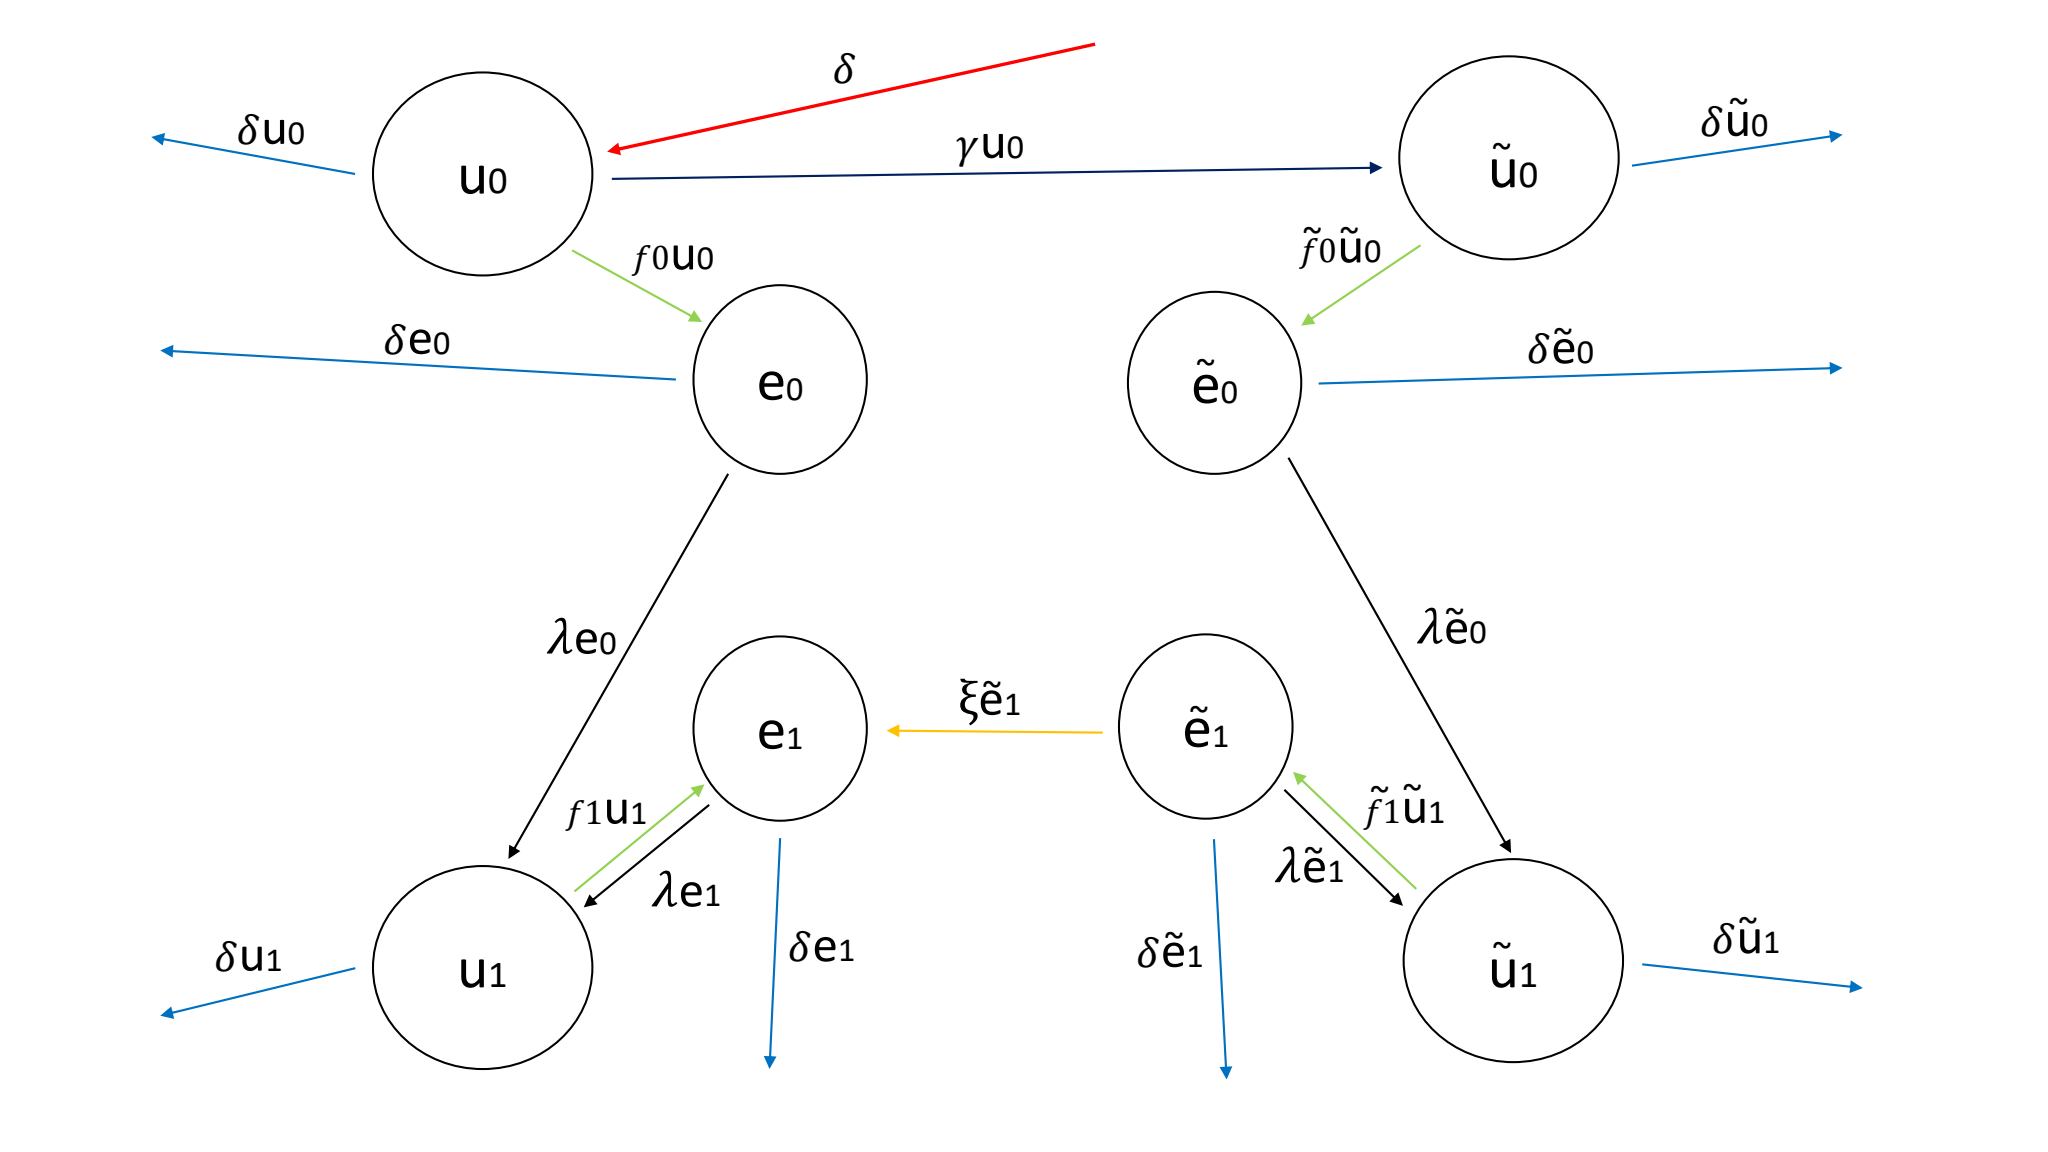
\includegraphics[width=1\linewidth]{figure_E2.png}
 \vspace{-1cm}
	\caption{Worker flows in and out of the various states when regaining skills is possible.}
	\label{figure regain skill}
\end{figure}

\subsection*{Beveridge curves}\label{regain beveridge}
With the visual help of Figure \ref{figure regain skill}, we can equate the flows in and out of each state, and after some algebra, we can show that the steady state measure of workers in the various states are as follows:
\begin{eqnarray}
u_0 &=& \frac{\delta}{\delta+\gamma+f_0}, \nonumber  \\
\tilde{u_0} &=& \frac{\gamma}{\delta+\Tilde{f_0}} \cdot  \frac{\delta}{\delta+\gamma+f_0},\nonumber  \\
e_0 &=& \frac{f_0}{\delta+\lambda} \cdot \frac{\delta}{\delta+\gamma+f_0}, \nonumber \\
\Tilde{e_0} &=& \frac{\Tilde{f_0}}{\delta+\lambda} \cdot \frac{\gamma}{\delta + \Tilde{f_0}} \cdot \frac{\delta}{\delta+\gamma+f_0},\nonumber   \\
 \tilde{u_1} &=& \frac{\lambda (\delta+\lambda+\xi) \tilde{f_0} \gamma \delta}{[\delta(\delta+\lambda+\xi)+\tilde{f_1}(\delta+\xi)](\delta+\lambda)(\delta+\tilde{f_0})(\delta+\gamma+f_0)}, \nonumber \\
  \tilde{e_1} &=& \frac{\tilde{f_1}\lambda \tilde{f_0} \gamma \delta}{[\delta(\delta+\lambda+\xi)+\tilde{f_1}(\delta+\xi)](\delta+\lambda)(\delta+\tilde{f_0})(\delta+\gamma+f_0)},  \nonumber  \\
  u_1 &=& \frac{\lambda}{(\gamma+\delta+f_0)(\delta+\lambda+f_1)}\left[f_0 + \xi \frac{\lambda \gamma \tilde{f_0} \tilde{f_1}}{[\delta(\delta+\lambda+\xi)+\tilde{f_1}(\delta+\xi)](\delta+\lambda)(\delta+\tilde{f_0})} \right],  \nonumber \\
  e_1 &=& \frac{1}{(\delta+\lambda)(\delta+\lambda+f_1)}\left[\frac{f_0f_1\lambda}{\delta+\gamma+f_0} + \xi \frac{(\delta+\lambda)(\delta+f_1)}{\delta} \tilde{e_1} \right]. \nonumber 
 \end{eqnarray}

\subsection*{Value Functions}\label{regain value functions}
We now move to the value functions starting with  firms. While we repeat all value functions for the reader's convenience, it is important to highlight that, under this extension, the only firm value function that will be different (from the main paper) is that of a firm employing a type-$\tilde{1}$ worker. Now, the value function of a vacant firm is given by:
\begin{equation}
   rV = -c + q_0 (J_0-V) + \Tilde{q_0}(\Tilde{J_0}-V) + q_1 (J_1-V) + \Tilde{q_1}(\Tilde{J_1}-V).\nonumber 
\end{equation}Free entry implies that in equilibrium we must have $V=0$, therefore, we can state the free entry condition as 
\begin{equation}
   c= q_0 J_0 + \Tilde{q_0}\Tilde{J_0} + q_1 J_1 + \Tilde{q_1}\Tilde{J_1}.\label{eq free entry regain} 
\end{equation}

We also have four value functions for productive firms in the various states, i.e., for firms that matched with the four different types of workers (type 0, $\tilde{0}$, 1, and $\tilde{1}$). These are given as follows:   
\begin{eqnarray}
    rJ_0 &=&p-\kappa-w_0-\lambda J_0 - \delta J_0,\nonumber  \\
    r\Tilde{J_0} &=&p-\kappa-\Tilde{\kappa}-\Tilde{w_0}-\lambda \Tilde{J_0} - \delta \Tilde{J_0},\nonumber\\
    rJ_1 &=&p-w_1-\lambda J_1 - \delta J_1, \nonumber \\
        r\Tilde{J_1} &=&p-\Tilde{\kappa}-\Tilde{w_1}-\lambda \Tilde{J_1} - \delta \Tilde{J_1} + \xi(J_1-\tilde{J_1}). \nonumber
    \end{eqnarray}As explained, all the functions are the same as before, except the last one.

We now move to the value functions for unemployed workers. All these functions are the same as in the baseline model: 
\begin{eqnarray}
    rU_0 &=& z+f_0(W_0-U_0)+\gamma(\Tilde{U_0}-U_0) - \delta U_0, \nonumber \\
    r\Tilde{U_0} &=& z+\Tilde{f_0}(\Tilde{W_0}-\Tilde{U_0})- \delta \Tilde{U_0}, \nonumber\\
    rU_1 &=& z+f_1(W_1-U_1)- \delta U_1, \nonumber\\
    r\Tilde{U_1} &=& z+\Tilde{f_1}(\Tilde{W_1}-\Tilde{U_1})- \delta \Tilde{U_1}.\nonumber 
\end{eqnarray}
The value functions for employed workers in the various states are given by: 
\begin{eqnarray}
    rW_0 &=&w_0+\lambda(U_1-W_0)- \delta W_0, \nonumber \\
     r\Tilde{W_0} &=& \Tilde{w_0}+\lambda(\Tilde{U_1}-\Tilde{W_0})- \delta \Tilde{W_0}, \nonumber\\
     rW_1 &=& w_1+\lambda(U_1-W_1)- \delta W_1, \nonumber \\
     r\Tilde{W_1} &=& \Tilde{w_1}+\lambda(\Tilde{U_1}-\Tilde{W_1})- \delta \Tilde{W_1} + \xi(W_1-\tilde{W_1}). \nonumber
     \end{eqnarray}
Notice that all these equations are the same as in the main body of the paper, except the last one, where the presence of the term multiplied by $\xi$ indicates the possibility that a type-$\tilde{1}$ worker can regain her skills later in her career. 


\subsection*{Wage Curves}\label{regain wage curves} 

The next task is to solve the bargaining problems in the various types of meetings and obtain the various wage curves. Following similar steps as in the main body of the paper, we arrive at the following wage equations: 

\noindent \textbf{Type $0: (1-\eta)(W_0-U_0) = \eta J_0$}
\begin{equation}\label{eq WC0 regain}
 \begin{split}
         w_0 & = \frac{r+\delta+\gamma +f_0}{r+\delta+\gamma+\eta f_0}\eta (p-\kappa) + \frac{(r+\lambda+\delta)(r+f_1+\delta)(r+\gamma+\delta)}{(r+\delta)(r+\delta+\gamma + \eta f_0)(r+\delta+\lambda+f_1)} (1-\eta) z + \\  
 & + \frac{\gamma \Tilde{f_0}\eta(p-\kappa-\Tilde{\kappa}-\Tilde{w_0})}{(r+\delta)(r+\delta+\gamma + \eta f_0)} - \frac{(1-\eta)\lambda f_1 (r+\gamma+\delta)w_1}{(r+\delta)(r+\delta+\gamma + \eta f_0)(r+\delta+\lambda+f_1)}. 
    \end{split}
\end{equation}
\textbf{Type $\Tilde{0}: (1-\eta)(\Tilde{W_0}-\Tilde{U_0}) = \eta \Tilde{J_0}$}
\begin{equation}
\begin{aligned}
    \Tilde{w_0} = 
    &\frac{1}{r+\delta+\eta \Tilde{f_0}}\Biggl\{ 
        (r+\delta+\Tilde{f_0})\eta(p-\kappa-\Tilde{\kappa}) + (r+\delta)(1-\eta)z \\
    &\quad - \frac{\lambda \eta \Tilde{f_1}}{r+\delta+\lambda+\xi} (p-\Tilde{\kappa}-\Tilde{w_1}) - \xi \frac{\lambda \Tilde{f_1} \eta}{(r+\delta+\lambda)(r+\delta+\lambda+\xi)} (p-w_1)
      \Biggr\}.\label{eq WC0 tilde regain}
\end{aligned}
\end{equation}
\textbf{Type 1: $(1-\eta)(W_1-U_1) = \eta J_1$}
\begin{equation}
 w_1 = \frac{\eta p (r+\lambda+\delta+f_1)+(1-\eta)z(r+\lambda+\delta)}{r+\lambda+\delta + \eta f_1}. \label{eq WC 1 regain}
 \end{equation}
 \textbf{Type $\Tilde{1}: (1-\eta)(\Tilde{W_1}-\Tilde{U_1}) = \eta \Tilde{J_1}$}
\begin{align}
% First line (no number)
\Tilde{w_1} 
&= \Biggl\{ 
    \bigl[(r+\delta)\,(r+\delta+\lambda+\xi+\Tilde{f_1}) + \xi\,\Tilde{f_1}\bigr]\,\eta\,(p-\Tilde{\kappa})
    + (1-\eta)\,z\,(r+\delta)\,(r+\lambda+\delta+\xi)
\nonumber \\[6pt]
% SECOND line: we tag (23) here
&\quad + \xi \,\frac{\Tilde{f_1}(r + \delta + \xi) - f_1(r + \delta + \lambda + \xi)}{r + \delta + \lambda}
         \,\eta\,(p - w_1) \Biggr\}\cdot
\label{eq WC1 tilde regain} \\[6pt]
% Third line (no number)
&\quad \frac{1}{
  (r + \delta)\,(r + \delta + \lambda + \xi)
  + \eta\,\Tilde{f_1}\,(r + \delta + \xi)
}.
\nonumber
\end{align}


\medskip


\subsection*{Definition of Steady State Equilibrium}\label{section definition of equil} 


\begin{definition}\label{definition equilibrium regain skill}
A steady state equilibrium in the model where type-$\tilde{1}$ workers stochastically regain skills later in their career is a list of wages for the four types of workers $(w_0, \Tilde{w_0}, w_1, \Tilde{w_1})$, a measure of vacant firms $v$, and measures of unemployed and employed workers in the various states $(u_0, \Tilde{u_0}, u_1, \Tilde{u_1}, e_0, \Tilde{e_0}, e_1, \Tilde{e_1})$, satisfying the free entry condition (\ref{eq free entry regain}), the four wage curves (\ref{eq WC0 regain}), (\ref{eq WC0 tilde regain}), (\ref{eq WC 1 regain}), and (\ref{eq WC1 tilde regain}), and the eight Beveridge curves reported earlier in this subsection. 
\end{definition} 


\subsection*{Quantitative Results} 

As we report in Section 1, the losses from early unemployment spells are large and persist for several years later in a worker's career; see \cite{wachter2020persistent} for a review of the empirical literature.
This motivated us to assume that the scarring effects of the skill shock $\gamma$ last for the whole career of a worker in the baseline model.
Indeed, \cite{rothstein2023lost} reports that the employment effects of high unemployment rates upon labor market entry are \textit{permanent}: cohorts that face high unemployment when they enter the labor market have lower employment rates throughout their careers.
However, it is useful to understand the quantitative impact of this assumption for the model implications.
To do so, we present the results of the Extension 1 model for various levels of the skill regaining parameter $\xi$.

\begin{table}[h!]
\begin{adjustbox}{width=0.8\columnwidth,center}

 \begin{tabular}{||c c c c c||} 
 \hline
 \\[-1.1em]
 \textbf{Variable} & \textbf{Baseline} & \textbf{Large $\xi$} & \textbf{Medium $\xi$} & \textbf{Small $\xi$}\\  
 \hline\hline
  $Y$  & 0.9379 & 0.9501 & 0.9486 & 0.9466 \\ 
  $u$  & 5.80\% & 5.98\% & 5.91\% & 5.84\%\\ 
  $f_{1}$  & 1.21 & 0.90 & 0.94 & 0.99\\ 
  $\tilde{f_{1}}$  & 0.51 & 0.44 & 0.45 & 0.47\\
  $f_{0}$  &  0.43 & 0.42 & 0.43 & 0.43\\
  $\tilde{f_{0}}$  & 0.42 & 0.41 & 0.42 & 0.42\\
  $w_{1}$  & 0.9852 & 0.9808 & 0.9814 & 0.9823\\
  $\tilde{w_{1}}$ & 0.9152 & 0.9006 & 0.9055 & 0.9090\\
  $w_{0}$  & 0.6620 & 0.7443 & 0.7254 & 0.7059\\
  $\tilde{w_{0}}$ & 0.7535 & 0.7475 & 0.7492 &  0.7508\\ [1ex] 
 \hline
 \end{tabular}
\end{adjustbox}
\centering
     \captionsetup{justification=centering}
\caption{Comparison of the Baseline Model with Extension 1 for various levels of $\xi$. Large $\xi$ implies an average employment duration of five years, medium $\xi$ of ten years, and small $\xi$ of twenty years until the worker regains their skill.} \label{table_ext1}
\end{table} 

Table \ref{table_ext1} summarizes the values of the main endogenous variables for the model of Extension 1, as well as the Baseline Model for comparison purposes.
We show the results for three levels of the skill regaining shock: $\xi = 1/(12*5)$ (``large $\xi$''),  $\xi = 1/(12*10)$ (``medium $\xi$''), and $\xi = 1/(12*20)$ (``small $\xi$'').
These values of $\xi$ imply different lengths of employment duration needed for the average worker's productivity to return to its initial level of $p$.
The large $\xi$ implies an average employment duration of five years, the medium $\xi$ of ten years, and the small $\xi$ of twenty years for skills to be regained.
Through the lens of the empirical literature, these three values are quite conservative: all studies surveyed by \cite{wachter2020persistent} report losses that persist for fifteen years after the worker's labor market entry, while \cite{arellano2022effect} reports effects on workers' skills that can be attributed to unemployment durations forty years earlier in a worker's career.
As $\xi$ becomes smaller, Extension 1 approaches the Baseline Model (the two are equivalent for $\xi = 0$).
Moreover, all variables move in the expected direction, approaching their baseline levels as the value of $\xi$ diminishes.

The impact of the value of $\xi$ on the economy's welfare is in the order 0.9 - 1.3\%.
In general, the magnitude of the effects for all variables is in the same order of magnitude as the policy interventions studied in the main body of the paper.
This is natural: the main economic trade-off of our paper lies in the skill loss of entrant workers while in unemployment.
Extension 1 makes this channel less severe by directly moving workers from the $\tilde{e}_{1}$ to the $e_{1}$ state.
The policy interventions studied in the paper lower the impact of the skill loss channel by raising the job-finding rate of entrant workers.
Thus, the quantitative impact of a larger $\xi$ is similar to increases in $f_{0}$ in the baseline model.
Indeed, one could interpret the model of Extension 1 as the outcome of an active labor market policy \citep{heckman1999economics} targeted to employed workers who have been through long unemployment spells early in their career.


\subsection{Extension 2: Gain experience while on first job}\label{section extension gain earlier experience}

The second assumption of the baseline model that we relax in this appendix is that young workers gain experience (only) after they lose their very first job. Specifically, we will adopt the milder assumption that workers who are employed at their first job can get hit by a shock and stochastically acquire experience while they are still holding that job. Workers who lose their first job before getting hit by that shock still become experienced, just like in the baseline model. Importantly, this new ``gain experience while on the first job shock" can hit workers who did not suffer skill loss during youth, as well as those who did suffer such skill loss. (We assume that the arrival rate of the shock is the same for both of these types.) In terms of the language developed in the paper, what is new here is that type-0 and type-$\tilde{0}$ workers may get hit by the Poisson shock $\zeta$ and become type-$1$ and type$\tilde{1}$ workers, respectively. Figure \ref{figure gain early experience} illustrates the worker flows in and out of every state in this new environment, and it is useful for deriving the Beveridge curves. The figure is identical to Figure 2 in the main paper, with the exception of the two new (orange) arrows pointing from the $e_0$ towards the $e_1$ bubble, and from the $\tilde{e}_0$ towards the $\tilde{e}_1$ bubble, indicating the newly introduced possibility of young workers gaining experience while they are still on their very first job. 

\begin{figure}
	\centering
	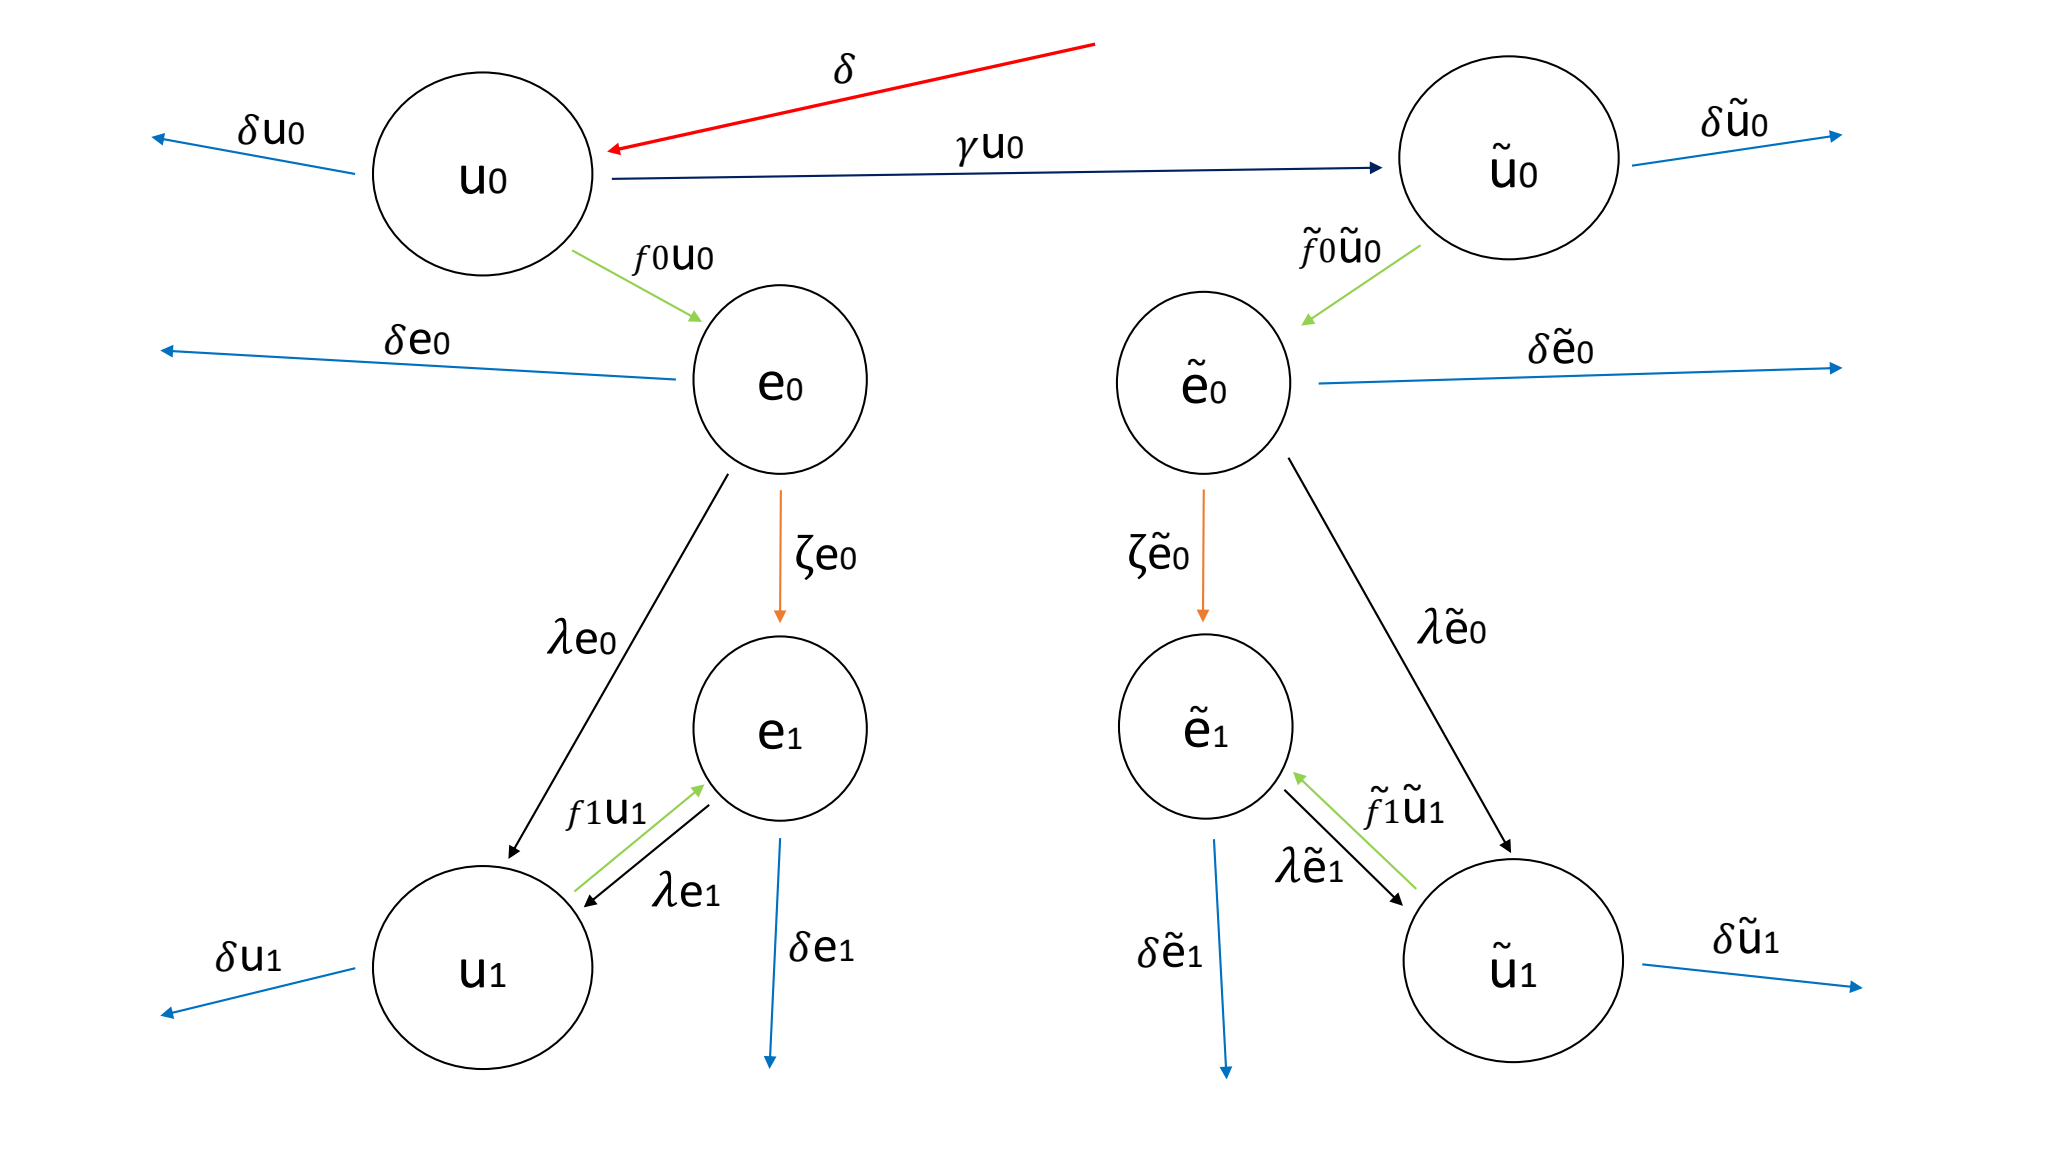
\includegraphics[width=1\linewidth]{figure_E1.png}
 \vspace{-1cm}
	\caption{Worker flows in and out of the various states when they can gain experience while on their first job.}
	\label{figure gain early experience}
\end{figure}

\subsection*{Beveridge curves}\label{regain beveridge}
With the visual help of Figure \ref{figure gain early experience}, we can equate the flows in and out of each state, and after some algebra, we can show that the steady state measure of workers in the various states are as follows:
\begin{eqnarray}
u_0 &=& \frac{\delta}{\delta+\gamma+f_0}, \nonumber  \\
\tilde{u_0} &=& \frac{\gamma}{\delta+\Tilde{f_0}} \cdot  \frac{\delta}{\delta+\gamma+f_0},\nonumber  \\
e_0 &=& \frac{f_0}{\delta+\lambda+\zeta} \cdot \frac{\delta}{\delta+\gamma+f_0}, \nonumber \\
\Tilde{e_0} &=& \frac{\Tilde{f_0}}{\delta+\lambda+\zeta} \cdot \frac{\gamma}{\delta + \Tilde{f_0}} \cdot \frac{\delta}{\delta+\gamma+f_0}, \nonumber  \\
 \tilde{u_1} &=& \frac{\lambda \Tilde{f_0} \gamma}{(\delta+\lambda+\Tilde{f_1})(\delta+\Tilde{f_0})(\delta+f_0+\gamma)},\nonumber  \\
  \tilde{e_1} &=& \frac{\Tilde{f_0} \gamma}{(\delta+\lambda)(\delta+f_0+\gamma)(\delta+\Tilde{f_0})} \left[\frac{\lambda \Tilde{f_1}}{\delta+\lambda+\Tilde{f_1}} + \frac{\zeta \delta}{\delta+\lambda+\zeta}\right],\nonumber    \\
  u_1 &=& \frac{\lambda}{\delta+f_1+\lambda}\frac{f_0}{\delta+f_0+\gamma}, \nonumber  \\
  e_1 &=& \frac{f_0}{(\delta+\lambda)(\delta+f_0+\gamma)}\left[\frac{\lambda f_1}{\delta+\lambda+f_1} +\frac{\zeta \delta}{\delta + \lambda + \zeta} \right]. \nonumber 
 \end{eqnarray}

\subsection*{Value Functions}
We now move to the value functions starting with  firms. The value function of a vacant firm is given by:
\begin{equation}
   rV = -c + q_0 (J_0-V) + \Tilde{q_0}(\Tilde{J_0}-V) + q_1 (J_1-V) + \Tilde{q_1}(\Tilde{J_1}-V).\nonumber 
\end{equation}
Free entry implies that in equilibrium we must have $V=0$, therefore, we can state the free entry condition as 
\begin{equation}
   c = q_0 J_0 + \Tilde{q_0}\Tilde{J_0} + q_1 J_1 + \Tilde{q_1}\Tilde{J_1}. \nonumber 
\end{equation}

We also have four value functions for productive firms in the various states, i.e., for firms that matched with the four different types of workers (type 0, $\tilde{0}$, 1, and $\tilde{1}$). These value functions are as follows: 
\begin{eqnarray}
    rJ_1 &=& p - w_1 - \lambda J_1 - \delta J_1, \nonumber \\
    r\Tilde{J_1} &=& p - \Tilde{\kappa} - \Tilde{w_1} - \lambda \Tilde{J_1} - \delta \Tilde{J_1}, \nonumber \\
    rJ_0 &=& p - \kappa - w_0 - \lambda J_0 - \delta J_0 + \zeta (J_1-J_0), \nonumber \\
    r\Tilde{J_0} &=& p - \kappa - \Tilde{\kappa} - \Tilde{w_0} - \lambda \Tilde{J_0} - \delta \Tilde{J_0} + \zeta (\Tilde{J_1}-\Tilde{J_0}).\nonumber 
\end{eqnarray}It is straightforward to notice that the first two are identical to the ones reported in the main paper, but the last two value functions are different, as is evident from the presence of the new shock $\zeta$. 

Next, consider the value functions of workers in the various states. The value functions for unemployed workers in the various states are identical to the ones reported in the main body of the paper and given by:
\begin{eqnarray}
    rU_0 &=& z + f_0 (W_0 - U_0) + \gamma (\Tilde{U_0} - U_0) - \delta U_0, \nonumber \\
    r\Tilde{U_0} &=& z + \Tilde{f_0} (\Tilde{W_0} - \Tilde{U_0}) - \delta \Tilde{U_0},\nonumber  \\
    rU_1 &=& z + f_1 (W_1 - U_1) - \delta U_1, \nonumber \\
    r\Tilde{U_1} &=& z + \Tilde{f_1} (\Tilde{W_1} - \Tilde{U_1}) - \delta \Tilde{U_1}.\nonumber 
\end{eqnarray}

For employed workers in the various states, we have:
\begin{eqnarray}
    rW_0 &=& w_0 + \lambda (U_1 - W_0) + \zeta(W_1-W_0) - \delta W_0 ,\nonumber  \\
    r\Tilde{W_0} &=& \Tilde{w_0} + \lambda (\Tilde{U_1} - \Tilde{W_0}) + \zeta(\Tilde{W_1}-\Tilde{W_0}) - \delta \Tilde{W_0}, \nonumber \\
    rW_1 &=& w_1 + \lambda (U_1 - W_1)-\delta W_1, \nonumber \\
    r\Tilde{W_1} &=& \Tilde{w_1} + \lambda (\Tilde{U_1} - \Tilde{W_1}) -\delta \Tilde{W_1}.\nonumber 
\end{eqnarray}
Again, it is obvious that the last two value functions are as in the main paper. However, the first two are different, with the term multiplied by $\zeta$ representing the possibility that inexperienced employed workers (with or without skill loss) can become experienced without having to go through unemployment first.  


\subsection*{Wage Curves}

The next task is to solve the bargaining problems in the various types of meetings and obtain the various wage curves. Following similar steps as in the main body of the paper, we arrive at the following wage equations: 

\medskip 

\noindent \textbf{Type 1: $(1-\eta)(W_1-U_1) = \eta J_1$}
\begin{equation}
 w_1 = \frac{\eta p (r+\lambda+\delta+f_1)+(1-\eta)z(r+\lambda+\delta)}{r+\lambda+\delta + \eta f_1}. \label{eq WC 1 early}
 \end{equation}
 \textbf{Type $\Tilde{1}: (1-\eta)(\Tilde{W_1}-\Tilde{U_1}) = \eta \Tilde{J_1}$}
\begin{equation}
\Tilde{w_1} = \frac{\eta (p-\Tilde{\kappa}) (r+\lambda+\delta+\Tilde{f_1})+(1-\eta)z(r+\lambda+\delta)}{r+\lambda+\delta + \eta \Tilde{f_1}}. \label{eq WC1 tilde early}
\end{equation}
\textbf{Type $\Tilde{0}: (1-\eta)(\Tilde{W_0}-\Tilde{U_0}) = \eta \Tilde{J_0}$}
\begin{equation}
\begin{aligned}
    \Tilde{w_0} = 
    & \frac{1}{r+\delta+\eta \Tilde{f_0}}\left\{ 
        (r+\delta+\Tilde{f_0})\eta(p-\kappa-\Tilde{\kappa}) + (1-\eta)z \left(r+\delta+\frac{(\lambda+\zeta)\Tilde{f_1}}{r+\lambda+\delta+\Tilde{f_1}}\right) \right. \\
    & \quad + \left. \frac{\eta \Tilde{f_0} \zeta (p-\Tilde{\kappa})}{r+\lambda+\delta} - \Tilde{w_1}\left(\frac{\eta \Tilde{f_0} \zeta}{r+\lambda+\delta} + \frac{(1-\eta)(\lambda+\zeta)\Tilde{f_1}}{r+\lambda+\delta+\Tilde{f_1}}\right)
      \right\}.\label{eq WC0 tilde early}
\end{aligned}
\end{equation}
\textbf{Type $0: (1-\eta)(W_0-U_0) = \eta J_0$}
\begin{align}
% First line (no number)
w_0
&=  \frac{1}{r+\delta+\gamma+\eta f_0} \Biggl\{ 
    (r+\delta+\gamma+f_0)\eta(p-\kappa) + \frac{(1-\eta)z}{r+\delta} \frac{[(r+\delta+f_1)(r+\delta+\lambda)+\zeta f_1](r+\delta + \gamma)}{r+\lambda+\delta+f_1}
\nonumber \\[6pt]
% SECOND line: we tag (23) here
&\quad + \eta f_0 \zeta \frac{p-w_1}{r+\delta+\lambda} + \frac{\eta \Tilde{f_0} \gamma}{r+\delta} (p-\kappa-\Tilde{\kappa}-\Tilde{w_0}) 
\label{eq WC0 early} \\[6pt]
% Third line (no number)
&\quad + \frac{\gamma \Tilde{f_0} \eta}{r+\delta} \zeta (p-\Tilde{\kappa} - \Tilde{w_1}) - \frac{(1-\eta)(\lambda+\zeta)(r+\delta+\gamma)}{r+\delta} f_1 \frac{w_1}{r+\lambda+\delta+f_1}
      \Biggr\}.
      \nonumber
\end{align}

\medskip


\subsection*{Definition of Steady State Equilibrium}\label{section definition of equil} 


\begin{definition}\label{definition equilibrium gain early}
A steady state equilibrium in the model where agents can gain experience while on their first job is a list of wages for the four types of workers $(w_0, \Tilde{w_0}, w_1, \Tilde{w_1})$, a measure of vacant firms $v$, and measures of unemployed and employed workers in the various states $(u_0, \Tilde{u_0}, u_1, \Tilde{u_1}, e_0, \Tilde{e_0}, e_1, \Tilde{e_1})$, satisfying the free entry condition, 
%(\ref{eq free entry regain}), 
the four wage curves (\ref{eq WC 1 early}), (\ref{eq WC1 tilde early}), (\ref{eq WC0 tilde early}), and (\ref{eq WC0 early}), and the eight Beveridge curves reported earlier in this subsection. 
\end{definition} 


\subsection*{Quantitative Results} 

Table \ref{table_ext2} summarizes the values of the main endogenous variables for the model of Extension 2, as well as the Baseline Model for comparison purposes.
We show the results for three levels of the experience gain shock: $\zeta = 1/12$ (``large $\zeta$''),  $\zeta = 1/15$ (``medium $\zeta$''), and $\zeta = 1/18$ (``small $\zeta$'').
These values of $\zeta$ imply different lengths for the duration of an entrant's first employment spell until the entrant becomes an experienced worker.
The large $\zeta$ implies an average employment duration of 12 months, the medium $\zeta$ of 15 months, and the small $\zeta$ of 18 months for the training costs to disappear.
In the model, the average job lasts for $1/\lambda \approx 20$ months.
As $\zeta$ becomes smaller, Extension 2 approaches the Baseline Model (the two are equivalent for $\zeta = 0$).
Moreover, all variables move in the expected direction, approaching their baseline levels as $\zeta$ becomes smaller.

The impact of the value of $\zeta$ on the economy's welfare is in the order 0.4 - 0.5\%, roughly half of the impact of Extension 1.
In general, larger values of $\zeta$ raise the average productivity of the unemployment pool and, as a result, firm entry and workers' job-finding rates.
Interestingly, the wages of type-0 workers plummet: employment in state $e_{0}$ is even more beneficial in the model of Extension 2, since workers can move to $e_{1}$ without an intervening unemployment spell.
As a result, entrant workers are willing to work for next to nothing just to improve their career prospects.
We should highlight that this result of Extension 2 has a flavor similar to the Internships intervention in the paper.
Moreover, the quantitative effects of Extension 2 are roughly in the same order of magnitude as the Internships scenario (which raised welfare by 0.62\%).

\begin{table}[h!]
\begin{adjustbox}{width=0.8\columnwidth,center}

 \begin{tabular}{||c c c c c||} 
 \hline
 \\[-1.1em]
 \textbf{Variable} & \textbf{Baseline} & \textbf{Large $\zeta$} & \textbf{Medium $\zeta$} & \textbf{Small $\zeta$}\\  
 \hline\hline
  $Y$  & 0.9379 & 0.9429 & 0.9424 & 0.9420 \\ 
  $u$  & 5.80\% & 4.98\% & 5.08\% & 5.14\%\\ 
  $f_{1}$  & 1.21 & 1.37 & 1.34 & 1.33\\ 
  $\tilde{f_{1}}$  & 0.51 & 0.59 & 0.58 & 0.57\\
  $f_{0}$  &  0.43 & 0.51 & 0.50 & 0.49\\
  $\tilde{f_{0}}$  & 0.42 & 0.50 & 0.49 & 0.48\\
  $w_{1}$  & 0.9852 & 0.9867 & 0.9866 & 0.9865\\
  $\tilde{w_{1}}$ & 0.9152 & 0.9178 & 0.9055 & 0.9176\\
  $w_{0}$  & 0.6620 & 0.0094 & 0.1170 & 0.2069\\
  $\tilde{w_{0}}$ & 0.7535 & 0.7502 & 0.7517 &  0.7522\\ [1ex] 
 \hline
 \end{tabular}
\end{adjustbox}
\centering
     \captionsetup{justification=centering}
\caption{Comparison of the Baseline Model with Extension 2 for various levels of $\zeta$. Large $\zeta$ implies an average employment duration of twelve months, medium $\zeta$ of fifteen months, and small $\zeta$ of eighteen months in their first job until an entrant worker becomes experienced.} \label{table_ext2}
\end{table} 


\subsection{Extension 3: Different bargaining powers based on experience}

As we explain in Section 2 of the paper, with the exception of productivity and the consequent differences in job-finding rates, all the other parameters of the model (including $\eta$, the bargaining power of the worker) are independent of the worker's type, and this is intentional. The goal of this modeling choice is to deliver results that are driven \textit{only} by differences in workers' experience, and whether they suffered skill loss during their youth, which is the focus of our paper. That said, it is not unreasonable to assume that workers of different (age and) experience may have different bargaining abilities. Therefore, in this subsection of the Web Appendix, we consider yet another extension of the baseline model, namely, one where experienced and inexperienced workers have different bargaining powers. Using our standard notation, we will let $\eta_0$ denote the bargaining power of inexperienced workers (types \(0\) and \(\tilde{0}\)), and $\eta_1$ the bargaining power of experienced workers (types \(1\) and \(\tilde{1}\)). (We assume that whether workers suffered skill loss or not during youth is irrelevant for their bargaining power; only experience matters.)  


Moving on to the analysis of the model, it is important to note that all Beveridge curves and all value functions remain unchanged compared to the baseline model. Only the structure of the bargaining problems in different types of meetings is modified, and this affects the derivation of the wage curves as shown below.

\subsection*{Bargaining problems}\label{section bargaining}

\noindent \textbf{Bargaining in a type-1 meeting}

\medskip

\noindent The standard Nash bargaining condition is:
\begin{equation}
(1-\eta_1)(W_1 - U_1) = \eta_1 \, J_1. \nonumber 
\end{equation}
Replacing $W_1$ and $J_1$ in the above, the type-1 wage can be written as
\[
w_1 \;=\; \eta_1 \, p + (1-\eta_1)\,z + \eta_1 \, f_1 \, J_1.
\]
Further substitution and rearrangement deliver the wage curve:
\begin{equation}
w_1 \;=\; \frac{\eta_1 \, p \,\bigl(r+\lambda+\delta+f_1\bigr)\;+\;\bigl(1-\eta_1\bigr)\,z\,\bigl(r+\lambda+\delta\bigr)}{r+\lambda+\delta\;+\;\eta_1\, f_1}.
\label{eq WC 1 mod}
\end{equation}
%Clearly, this is a relationship between the wage for type-1 workers and their job arrival rate, which, in turn, depends on firm entry and market tightness. 

\bigskip 
\noindent \textbf{Bargaining in a type-$\tilde{1}$ meeting}

\medskip

\noindent The standard Nash bargaining condition is:
\begin{equation}
(1-\eta_1)\bigl(\tilde{W_1} - \tilde{U_1}\bigr) \;=\; \eta_1 \,\tilde{J_1}.\nonumber 
\end{equation}
By substituting the relevant value functions and rearranging, the wage curve for type-$\tilde{1}$ workers is:
\begin{equation}
\tilde{w_1} 
\;=\; \frac{\eta_1 \,\bigl(p - \tilde{\kappa}\bigr)\bigl(r+\lambda+\delta+\tilde{f_1}\bigr)
\;+\;\bigl(1-\eta_1\bigr)\,z\,\bigl(r+\lambda+\delta\bigr)}
{r+\lambda+\delta\;+\;\eta_1\,\tilde{f_1}}.
\label{eq WC 1 tilde mod}
\end{equation}
\bigskip 

\noindent \textbf{Bargaining in a type-$\tilde{0}$ meeting}

\medskip

\noindent The standard Nash condition is:
\[
(1-\eta_0)\bigl(\tilde{W_0} - \tilde{U_0}\bigr) \;=\; \eta_0 \,\tilde{J_0},
\]
which leads to the following wage curve for type-$\tilde{0}$ workers:
\begin{equation} 
\label{eq WC0 tilde mod}
\begin{split}
\tilde{w_0} \;=\; \frac{1}{r+\delta+\eta_0 \,\tilde{f_0}}
\Bigl[
&\,\eta_0\,\bigl(p-\kappa-\tilde{\kappa}\bigr)\,\bigl(r+\delta+\tilde{f_0}\bigr) \\
&\quad+\;\frac{\bigl(r+\delta+\lambda\bigr)\bigl(r+\delta+\tilde{f_1}\bigr)}{r+\delta+\lambda+\tilde{f_1}}\,(1-\eta_0)\,z \\
&\quad-\;\frac{\lambda\,(1-\eta_0)\,\tilde{f_1}}{r+\delta+\lambda+\tilde{f_1}}\;\tilde{w_1}
\Bigr].
\end{split}
\end{equation}

\bigskip

\noindent \textbf{Bargaining in a type-0 meeting}

\medskip

\noindent The standard Nash condition here is:
\[
(1-\eta_0)\bigl(W_0 - U_0\bigr) \;=\; \eta_0\,J_0,
\]
which yields the wage curve for type-0 workers:
\begin{equation}\label{eq WC0 mod}
\begin{split}
w_0 \;=\;& \frac{r+\delta+\gamma+f_0}{r+\delta+\gamma+\eta_0\,f_0}\;\eta_0\,(p-\kappa) \\
&\;+\;\frac{(r+\lambda+\delta)\,(r+f_1+\delta)\,(r+\gamma+\delta)}{(r+\delta)\,\bigl(r+\delta+\gamma+\eta_0\,f_0\bigr)\,\bigl(r+\delta+\lambda+f_1\bigr)}\,(1-\eta_0)\,z \\  
&\;+\;\frac{\gamma\,\tilde{f_0}\,\eta_0\,\bigl(p-\kappa-\tilde{\kappa}-\tilde{w_0}\bigr)}{(r+\delta)\,\bigl(r+\delta+\gamma+\eta_0\,f_0\bigr)} \\
&\;-\;\frac{(1-\eta_0)\,\lambda\,f_1\,(r+\gamma+\delta)\,w_1}{(r+\delta)\,\bigl(r+\delta+\gamma+\eta_0\,f_0\bigr)\,\bigl(r+\delta+\lambda+f_1\bigr)}.
\end{split}
\end{equation}

\subsection*{Definition of Steady State Equilibrium}

\noindent A steady state equilibrium for this version of the model is a list of wages 
$
\bigl(w_0, \tilde{w_0}, w_1, \tilde{w_1}\bigr),
$
a measure of vacant firms \(v\), and measures of unemployed and employed workers in all states,
$
\bigl(u_0, \tilde{u_0}, u_1, \tilde{u_1}, e_0, \tilde{e_0}, e_1, \tilde{e_1}\bigr),
$
satisfying the free-entry condition, the four wage curves \eqref{eq WC 1 mod}, \eqref{eq WC 1 tilde mod}, \eqref{eq WC0 tilde mod}, and \eqref{eq WC0 mod}, and the standard Beveridge curves (i.e., the ones described in Section 3.1 of the main paper).


\subsection*{Quantitative Results} 

Table \ref{table_ext3} summarizes the values of the main endogenous variables for the model of Extension 3, as well as the Baseline Model for comparison purposes.
We show the results for two combinations of bargaining power parameters: i) $\eta_{0}=\alpha/2$, $\eta_{1} = \alpha$ and ii) $\eta_{0}=\alpha$, $\eta_{1} = \alpha/2$ (as a reminder, $\eta_{0}= \eta_{1} = \alpha$ in the baseline model).
The first combination corresponds to a scenario in which entrants have lower bargaining power than experienced workers,  while the second combination to the opposite case.
In general, the empirical evidence on the bargaining power over a worker's life-cycle is not conclusive.
As one can infer from the work of \cite{cordoba2023endogenous}, there are factors that point to a lower bargaining power early (e.g., lower human capital) or later (e.g., retirement) in a worker's career.
Hence, we show the model implications for both scenarios (interpreting entrants as younger and the experienced ones as older workers).

The first implication of Table \ref{table_ext3} is that the impact of changes in workers' bargaining power has very modest effects on welfare.
The overall effects are an order of magnitude smaller than the effects predicted by the models of Extensions 1 and 2.
In general, smaller values of $\eta$'s raise the fraction of the surplus received by the firms and, as a result, firm entry and workers' job-finding rates.
Similar to Extension 2, the wages of type-0 workers decrease following the exact same reasoning.
Comparing the different bargaining power combinations, welfare's behavior is non-linear: it increases when $\eta_{0}$ decreases but it actually decreases when $\eta_{1}$ decreases.
The economics here follows the well-known reasoning of \cite{hosios1990efficiency}, according to which unemployment may be inefficiently low if workers' bargaining power is below some threshold value, because of the large costs of vacancy creation due to inefficiently high firm entry.


\begin{table}[h!]
\begin{adjustbox}{width=0.9\columnwidth,center}

 \begin{tabular}{||c c c c||} 
 \hline
 \\[-1.1em]
 \textbf{Variable} & \textbf{Baseline} & $\eta_{0}=\alpha/2$, $\eta_{1} = \alpha$ & $\eta_{0}=\alpha$, $\eta_{1} = \alpha/2$\\  
 \hline\hline
  $Y$  & 0.9379 & 0.9385 & 0.9364\\ 
  $u$  & 5.80\% & 4.91\% & 3.74\% \\ 
  $f_{1}$  & 1.21 & 1.38 & 1.73 \\ 
  $\tilde{f_{1}}$  & 0.51 & 0.60 & 0.78\\
  $f_{0}$  &  0.43 & 0.52 & 0.69 \\
  $\tilde{f_{0}}$  & 0.42 & 0.51 & 0.67\\
  $w_{1}$  & 0.9852 & 0.9869 & 0.9701\\
  $\tilde{w_{1}}$ & 0.9152 & 0.9184 & 0.8927 \\
  $w_{0}$  & 0.6620 & 0.4870 & 0.7069\\
  $\tilde{w_{0}}$ & 0.7535 & 0.7097 & 0.7648\\ [1ex] 
 \hline
 \end{tabular}
\end{adjustbox}
\centering
     \captionsetup{justification=centering}
\caption{Comparison of the Baseline Model with Extension 3 for various levels of $\eta_{0}$ and $\eta_{1}$.} \label{table_ext3}
\end{table} 
 


\setlength{\bibsep}{0pt}

\bibliography{AGKbib} 


\end{document}
